%
% Simple template for generating drafts of papers and articles
%
\documentclass[12pt,]{article}
\usepackage{authblk}
\usepackage{fullpage}
\usepackage{amssymb,amsmath}
\usepackage[utf8x]{inputenc}
\usepackage[T1]{fontenc}
\usepackage{siunitx}
\usepackage[version=3]{mhchem}
\usepackage{bm}
\usepackage{multirow}

\usepackage{natbib}
\bibliographystyle{genetics}

% \pagestyle{empty} % if suppressing page numbers

% to add line numbers
%\usepackage[left]{lineno}
%\linenumbers

\usepackage{setspace}
\onehalfspacing

\usepackage[unicode=true]{hyperref}
\hypersetup{breaklinks=true,
            bookmarks=true,
            colorlinks=false,
            pdfborder={0 0 0}}
\urlstyle{same} % don't use a different (monospace) font for urls

\setcounter{secnumdepth}{5}

\usepackage{graphicx}
\graphicspath{{figures/}}
% Redefine \includegraphics so that, unless explicit options are
% given, the image width will not exceed the width or the height of the page.
% Images get their normal width if they fit onto the page, but
% are scaled down if they would overflow the margins.
\makeatletter
\def\ScaleWidthIfNeeded{%
 \ifdim\Gin@nat@width>\linewidth
    \linewidth
  \else
    \Gin@nat@width
  \fi
}
\def\ScaleHeightIfNeeded{%
  \ifdim\Gin@nat@height>0.9\textheight
    0.9\textheight
  \else
    \Gin@nat@width
  \fi
}
\makeatother
\setkeys{Gin}{width=\ScaleWidthIfNeeded,height=\ScaleHeightIfNeeded,keepaspectratio}%

\newcommand{\beginsupplement}{%
        \setcounter{table}{0}
        \renewcommand{\thetable}{S\arabic{table}}%
        \setcounter{figure}{0}
        \renewcommand{\thefigure}{S\arabic{figure}}%
        \setcounter{equation}{0}
        \renewcommand{\theequation}{S\arabic{equation}}
     }

%%%%%%%%%%%%%%%%%%%%%%%%%%%%%%%%%%%%%%%%%%%%%%%%%%%%%%%%%%%%%%%%%%%%%%%%%%%%%%

\title{\textbf{Detecting frequency-dependent selection through the effects of genotype similarity on fitness components}\thanks{This is the peer-reviewed version of the following article: Sato Y. et al., (2023) Detecting frequency-dependent selection through the effects of genotype similarity on fitness components. \textit{Evolution}. \url{https://doi.org/10.1093/evolut/qpad028}; This post-print may be used for non-commercial purposes in accordance with Oxford University Press's Terms and Conditions for Use of Self-Archived Versions; This is not the published version. Please cite only the published version.}}
\author[1,2]{Yasuhiro Sato\thanks{Co-correspondence: yasuhiro.sato@uzh.ch (email); +41 44 635 4970 (phone)}}
\affil[1]{Department of Evolutionary Biology and Environmental Studies, University of Zurich, Winterthurerstrasse 190, 8057 Zurich, Switzerland}
\affil[2]{Research Institute for Food and Agriculture, Ryukoku University, Yokotani 1-5, Seta Oe-cho, Otsu, Shiga 520-2194, Japan}
\author[3]{Yuma Takahashi}
\affil[3]{Graduate School of Science, Chiba University, Yayoi-cho 1-33, Inage-ku, Chiba 263-8522, Japan}
\author[1]{Chongmeng Xu}
\author[1,4]{Kentaro K. Shimizu\thanks{Co-correspondence: kentaro.shimizu@uzh.ch (email); +41 44 635 6740 (phone)}}
\affil[4]{Kihara Institute for Biological Research, Yokohama City University, Maioka 641-12, Totsuka-ward, Yokohama 244-0813, Japan}

\date{\today}

%%%%%%%%%%%%%%%%%%%%%%%%%%%%%%%%%%%%%%%%%%%%%%%%%%%%%%%%%%%%%%%%%%%%%%%%%%%%%%

\begin{document}

\maketitle

\newpage

\section*{Abstract}
Frequency-dependent selection (FDS) is an evolutionary regime that can maintain or reduce polymorphisms. Despite the increasing availability of polymorphism data, few effective methods are available for estimating the gradient of FDS from the observed fitness components. We modeled the effects of genotype similarity on individual fitness to develop a selection gradient analysis of FDS. This modeling enabled us to estimate FDS by regressing fitness components on the genotype similarity among individuals. We detected known negative FDS on the visible polymorphism in a wild \textit{Arabidopsis} and damselfly by applying this analysis to single-locus data. Further, we simulated genome-wide polymorphisms and fitness components to modify the single-locus analysis as a genome-wide association study (GWAS). The simulation showed that negative or positive FDS could be distinguished through the estimated effects of genotype similarity on simulated fitness. Moreover, we conducted the GWAS of the reproductive branch number in \textit{Arabidopsis thaliana} and found that negative FDS was enriched among the top-associated polymorphisms of FDS. These results showed the potential applicability of the proposed method for FDS on both visible polymorphism and genome-wide polymorphisms. Overall, our study provides an effective method for selection gradient analysis to understand the maintenance or loss of polymorphism. 

\medskip
\noindent
\textbf{Running title:} Detecting frequency-dependent selection

\medskip
\noindent
\textbf{Keywords:} Frequency-dependent selection, Genome-wide association study, Selection gradient analysis


\newpage

\section{Introduction}
Wild organisms possess naturally occurring polymorphisms in their genomes. Polymorphisms, i.e., multiple alleles at a single locus, can be maintained by several forms of balancing selection such as through negative frequency-dependent selection (FDS), overdominance, and spatiotemporal variation in selection pressure \citep{hedrick2007balancing}. Among these mechanisms, negative FDS can maintain multiple alleles at a locus by favoring rare alleles over common alleles; this regime has been reported to maintain polymorphisms in many traits such as coloration \citep{gigord2001negative, takahashi2010negative, le2015evolutionary, nosil2018natural}, self-incompatibility \citep{llaurens2008does, joly2011migration, shimizu2015evolution}, and resistance to natural enemies \citep{antonovics1984experimental, brunet2000disease, sato2017herbivore}. Conversely, positive FDS unbalances polymorphisms by favoring common alleles over rare alleles \citep{borer2010positive, garrido2016effect}. These actions of FDS can modulate population-level processes such that the population-level mean fitness may increase or decrease as a consequence of negative or positive FDS, respectively \citep{takahashi2014evolution,svensson2019frequency}. 

Thus far, many researchers have attempted to quantify a gradient of natural selection by regressing fitness components on the traits of interests \citep[e.g.,][]{lande1983measurement, heisler1987method, mitchell1987regression, chong2018note}. This framework of selection gradient analysis \citep{lande1983measurement} is also applicable to FDS. Several studies included population-level genotype frequencies as a covariate in the selection gradient analysis to reveal how observed fitness components depended on genotype frequencies \citep{mccauley1998frequency, calsbeek2010geographic, sato2017herbivore}. However, this approach is not technically efficient because we need to separately analyze the fitness-frequency relationship for each genotype. If the entire dataset is separated into subset data of each genotype, this reduces the total sample size and thus decrease statistical power to detect FDS. Therefore, a simpler regression model is required to quantify FDS in the framework of selection gradient analysis.

Besides its conventional usage, selection gradient analysis can also be applied for single nucleotide polymorphism (SNP) data for quantifying natural selection at a genome-wide scale \citep{durham_genome-wide_2014, fisher_genetic_2016, exposito2019natural}. For example, \cite{exposito2019natural} quantified directional selection in the genome of \textit{Arabidopsis thaliana} by conducting the selection gradient analysis for all SNPs. In technical contexts, the statistical genetic models of genome-wide association studies (GWASs) and quantitative trait locus (QTL) mapping are based on the linear regressions of a trait on genotype values \citep{broman2009single, gondro2013genome}. If the target trait is a direct component of fitness, the regression coefficient of each locus describes the relationship between individual's fitness and character --- that is, selection gradient \citep{lande1983measurement} --- at a target locus. However, few methods, if any, can be used to detect FDS from GWAS or QTL mapping data. 

Population genetics theory has long modeled genotype’s fitness as a product of the frequency of a focal genotype and its encounter frequency with the other genotypes to develop a general model of FDS \citep{wright1948roles, clarke1964frequency, schutz1969inter, cockerham1972frequency, asmussen_frequency-dependent_1990, trotter2007frequency, schneider_maximization_2008}. Such a population genetic model of FDS was indeed used in the empirical analyses of inter-genotype competition in plants \citep{schutz1969inter} and insects \citep{alvarez2005models}. Empirical evidence further suggests that FDS occurs not only through direct competitions but also through indirect interactions between genotypes \citep{antonovics1984experimental,gigord2001negative,takahashi2010negative,sato2017herbivore}. For example, natural enemies mediate negative FDS on plant resistance when they attack undefended plants surrounding defended plants \citep{antonovics1984experimental, brunet2000disease, sato2017herbivore}. In this case, FDS is expected to occur within a local plant patch or among neighboring plants \citep[][cf. Fig. \ref{fig1:scheme}a bottom]{janzen1970herbivores, connell1971role, molofsky2001coexistence, browne2016frequency}. Further, mate choice in male insects mediates negative FDS on female color polymorphism when male insects learn about different colors of female individuals \citep{van2001frequency,takahashi2010negative}. These individual insects are likely to move and interact within experimental cages or subpopulations under FDS \citep[][cf. Fig. \ref{fig1:scheme}a top]{cosmidis1999rarer,fitzpatrick2007maintaining,takahashi2014evolution}. If the population genetic model of FDS can be transformed as a general regression model, the selection gradient analysis of FDS will become feasible in diverse organisms under various spatial structures (Fig. \ref{fig1:scheme}a).

\begin{figure}[ht]
  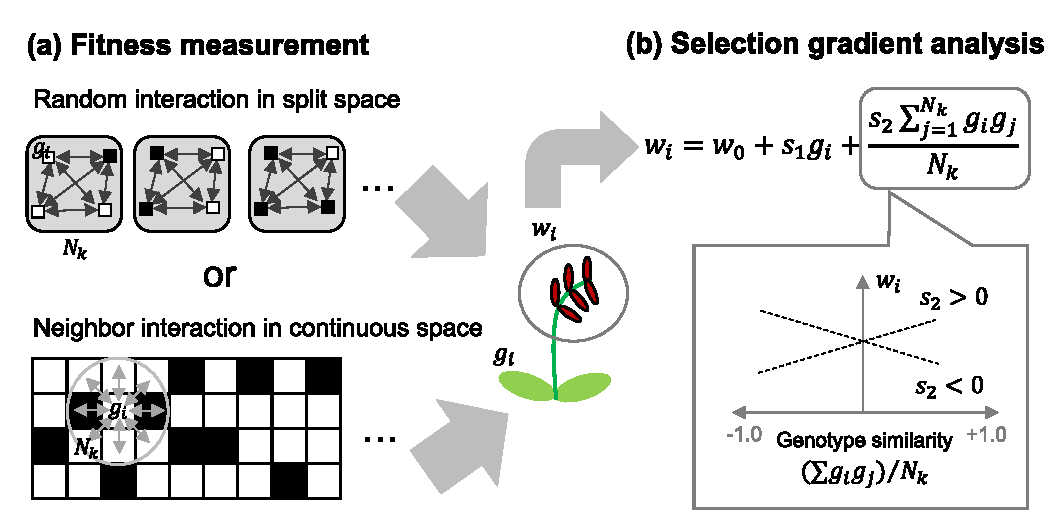
\includegraphics[width=\linewidth]{scheme.pdf}
  \caption{Workflow from the fitness measurement (a) to selection gradient analysis (b). (a) Individual fitness is observed as a consequence of interactions (two-way arrows) among individuals carrying different genotypes (black and white squares) within split subpopulations (top gray squares: cf. the case of \textit{A. halleri} and \textit{I. elegans} in this study) or a continuous space (bottom: cf. the case of \textit{A. thaliana}). (b) The selection gradient is then analyzed based on regression of the observed fitness $w_i$ on genotypes $g_i$. The second term in the equation is the same as that in Equation (\ref{eq:1}) and indicates how the second selection coefficient $s_2$ represents the effects of genotype similarity between the genotypes $g_i$ and $g_j$. Summation $\sum$ is made over $N_k$ potentially interacting neighbors with the genotype $g_j$ where $j = 1 ... N_k$.
}
  \label{fig1:scheme}
\end{figure}

In this study, we propose an effective regression model that infers FDS based on observed fitness. The key idea behind our statistical modeling is the inclusion of genotype similarity as a covariate in selection gradient analyses (see methods "\textbf{Model development}"). We tested whether the proposed regression model (i) can accurately detect known FDS on a single-locus polymorphism (see the methods and results "\textbf{Single-locus examples}") and (ii) screen FDS-associated polymorphisms from genome-wide SNPs (see the methods and results "\textbf{GWAS extension}") to demonstrate the potential applicability of our methodology. For (i) the single-locus analyses, we reanalyzed data from previous studies on herbivore-mediated negative FDS on the trichome dimorphism of a wild herb \textit{Arabidopsis halleri} \citep{sato2017herbivore} and male-mediated negative FDS on the female color polymorphism of a damselfly \textit{Ischnura elegans} \citep{takahashi2014evolution}. For (ii) the genome-wide extension, we combined simulations and empirical \textit{A. thaliana} data to showcase the GWAS of FDS. These empirical investigations on various systems will help illustrate the potential applicability of our regression method as a selection gradient analysis of FDS.

\section{Methods}

\subsection{Model development}
We analyzed the effects of genotype similarity on individual fitness to develop a simple regression model of FDS. We first modeled FDS based on genotype similarity among individuals (see "\textit{\textbf{FDS model based on genotype similarity}}" below), and then, we redefined it as a regression model (see "\textit{\textbf{Regression model of FDS}}" below). We finally analyzed fitness functions under the assumption of a panmictic population to illustrate how regression coefficients infer negative or positive FDS (see "\textit{\textbf{Fitness functions given by regression coefficients}}" below).

\subsubsection{FDS model based on genotype similarity}
We focused on the effects of genotype similarity on individual fitness to model interactions between genotypes. Let us assume that diploid organisms interact within panmictic subpopulations and produce their offspring based on the realized fitness (Fig. \ref{fig1:scheme}a top). We assume that a subpopulation $k$ belongs to the meta-population $K$ as $k \in K$, where two individuals $i$ and $j$ belong to subpopulation $k$ such that $i,j \in k$. We further assume that individuals $i$ and $j$ have two alleles at a locus, with the ancestral allele A being dominant over the derived allele a, where genotype values are encoded as $g_i \in$ \{AA, Aa, aa\} $=$ \{+1, +1, -1\}. This dominant encoding represents well-reported cases in which FDS often acts on a trait exhibiting dimorphism under Mendelian inheritance with complete dominance \citep[e.g.,][]{takahashi2010negative,sato2017herbivore}. We modeled fitness $w$ for individual $i$ by incorporating the genotype similarity between $i$ and $j$ as 

\begin{equation}
w_i = w_0 + s_1 g_i + \frac{s_2}{N_k}\sum^{N_{k}}_{j=1}{g_ig_j}\label{eq:1}
\end{equation}
\noindent
where $w_0$ represents the base fitness; $s_1$ and $s_2$ represent the selection coefficients for individual genotype effects and genotype similarity, respectively; and $N_k$ represents the total number of individuals within subpopulation $k$. The term $\sum^{N_{k}}_{j=1}{g_ig_j}$ represents the average similarity (or difference) of the genotype composition of the subpopulation (or neighbors) from the individual $i$. If two individuals share the \textit{same} genotype values, $g_ig_j = (+1)\times(+1) = (-1)\times(-1) = +1$. If two individuals have \textit{different} genotype values, $g_ig_j = (-1)\times(+1) = (+1)\times(-1) = -1$. Thus, the within-population genotype similarity $(\sum^{N_{k}}_{j=1}{g_ig_j})/N_k$ ranges from -1.0 (perfect dissimilarity) to +1.0 (perfect similarity; Fig. \ref{fig1:scheme}b) as a mean similarity across the number of interacting individuals within the subpopulation $N_k$. This line of modeling has a similar structure with the Ising model of statistical physics (Appendix S1; Table \ref{tableS1:MCMCinherit}; and Fig. \ref{figS1:Ising}), where positive or negative $s_2$ favors the same or different genotypes between individuals $i$ and $j$ \citep{sato2019neighbor}. Alternatively, we can also assume an additive expression for a trait responsible for FDS as $g_i \in$ \{AA, Aa, aa\} $=$ \{+1, 0, -1\}, where the products involving heterozygotes were considered $0 \times 0 = 0$ (neither similar nor dissimilar). This additive encoding assumes the intermediate strength of FDS for an intermediate morph (Appendix S2; Fig. \ref{figS2:FDSadd}). However, most empirical studies have reported FDS between two out of multiple morphs \citep[e.g.,][]{gigord2001negative,takahashi2010negative,le2015evolutionary,sato2017herbivore,nosil2018natural}. As the intermediate FDS on an additive trait is still uncommon, we focused on dominant encoding.

\subsubsection{Regression model of FDS}
We modified Equation (\ref{eq:1}) as a regression model to fit the proposed model to empirical data. We redefined the individual fitness $w_i$ as the response variable $y_i$; the genotype $g_i$ as the explanatory variables $x_i$; the base fitness $w_0$ as the intercept $\beta_0$; and the selection coefficients $s_1$ and $s_2$ as the regression coefficients $\beta_1$ and $\beta_2$, respectively. Further, we added a residual error $e_i$ to Equation (\ref{eq:1}) to obtain the statistical model 

\begin{equation}
y_i = \beta_0 + \beta_1x_i + \frac{\beta_2}{N_k}\sum^{N_{k}}_{j=1}{x_ix_j} + e_i \label{eq:2}
\end{equation}
\noindent
where Equation (\ref{eq:2}) poses a regression analysis to estimate $\hat{\beta}_1$ and $\hat{\beta}_2$ from the given $y_i$ and $x_i$. According to the inference from $s_2$ (Appendix S1), negative or positive $\beta_2$ represents a negative or positive FDS between two alleles as analyzed below (see "\textit{\textbf{Fitness functions given by regression coefficients}}"). The negative fitness effects on one allele coincide with positive effects on another allele when $y_i$ is a relative fitness, and therefore, it would not be necessary to consider the asymmetric FDS described in the next paragraph.

When $y_i$ is measured as an absolute fitness, the FDS may act asymmetrically between the two alleles. For example, negative FDS on relative fitness is known to exist in the Hawk--Dove game, where both hawks and doves suffer from intensified competition with hawks. Therefore, a reduction of absolute fitness is observed along increasing frequencies of hawks \citep[][see also Fig. \ref{figS3:FDSinbred}b]{takahashi2018balanced}. We modified Equation (\ref{eq:2}) to distinguish the asymmetric and symmetric FDS from absolute fitness. The asymmetric FDS can be modeled by a multiplicative interaction term between the second and third terms of Equation (\ref{eq:2}) \citep{sato2019neighbor}; it is expressed as 

\begin{equation}
y_i = \beta_0 + \beta_1x_i + \frac{\beta_2}{N_k}\sum^{N_{k}}_{j=1}{x_ix_j} + \frac{\beta_{12}x_i}{N_k}\sum^{N_{k}}_{j=1}{x_ix_j} + e_i \label{eq:3}
\end{equation}
\noindent
where $\beta_{12}$ indicates the coefficient for the asymmetric effects of genotype similarity. If $\beta_{12}$ was statistically significant, the slope coefficient of the genotype similarity differed among focal genotypes \citep{sato2019neighbor}, which means that the strength or direction of FDS is asymmetric between genotypes. A practical usage of Equation (\ref{eq:3}) is the same as the test of an interaction term in a standard regression model: We should first test $\beta_{12}$ using Equation (\ref{eq:3}) and then test $\beta_2$ using the linear model Equation (\ref{eq:2}) if $\beta_{12}$ is not significant.

\subsubsection{Fitness functions given by regression coefficients}
We analyzed Equation (\ref{eq:3}) as a function of allele frequencies to clarify how the coefficients for genotype similarity effects $\beta_2$ and asymmetric effects $\beta_{12}$ corresponded to FDS. If we suppose that all individuals uniformly interact in a sufficiently large population with random mating (i.e., $N_k \to \infty$), the probability of one genotype interacting with the other genotypes depends on genotype frequencies derived from an allele frequency within a population (Appendix S2). Let $f$ be the frequency of the A allele within the panmictic infinite population. The ratio of genotype frequency on panmixia was given as follows: AA: Aa: aa = $f^2:2f(1-f):(1-f)^2$. Assuming the complete dominance of the A allele over the a allele ($x_i \in$ \{AA, Aa, aa\} $=$ \{+1, +1, -1\}), we then calculated all the combinations among the three genotypes (Table \ref{tableS2:intTable}) and consequent fitness $y_i$ for AA, Aa, and aa genotypes as

\begin{subequations}
\begin{align}
y_\mathrm{AA} = y_\mathrm{Aa} = \beta_0 + (\beta_2 + \beta_{12})f^2 + 2(\beta_2 + \beta_{12}) f(1-f) - (\beta_2 + \beta_{12})(1-f)^2 \label{eq:4a} \\
y_\mathrm{aa} = \beta_0 - (\beta_2 - \beta_{12}) f^2 - 2(\beta_2 - \beta_{12})f(1-f) + (\beta_2 - \beta_{12})(1-f)^2 \label{eq:4b}
\end{align}
\end{subequations}
\noindent
where $y_\mathrm{AA}$, $y_\mathrm{Aa}$, and $y_\mathrm{aa}$ represent the fitness values for the AA, Aa, and aa genotypes, respectively (Appendix S2). The allele-level fitness was then defined by weighting the genotype fitness with the allele frequency as follows:

\begin{subequations}
\begin{align}
y_\mathrm{A} = f y_\mathrm{AA} + (1 - f) y_\mathrm{Aa} \label{eq:5a} \\
y_\mathrm{a} = f y_\mathrm{Aa} + (1 - f) y_\mathrm{aa} \label{eq:5b}
\end{align}
\end{subequations}

\noindent
In Equations (4) and (5), the sign of the symmetric effects $\beta_2$ represents negative or positive FDS on relative fitness between two alleles, while the asymmetric effects $\beta_{12}$ determine the slope of absolute fitness along the allele frequency $f$. Figure \ref{fig2:asym} shows how the fitness values Equations (\ref{eq:5a}) and (\ref{eq:5b}) vary in response to $f$. Symmetric negative FDS was exemplified by the negative $\beta_2$ without any asymmetric effects $\beta_{12}$ (i.e., $\beta_{12}=0$; Fig. \ref{fig2:asym}a). Asymmetric negative FDS was described by the negative (Fig. \ref{fig2:asym}b) or positive (Fig. \ref{fig2:asym}c) asymmetric effect $\beta_{12}$, where the negative $\beta_2$ denoted negative FDS on the relative fitness between two alleles (Fig. \ref{fig2:asym}b and c). In contrast, symmetric positive FDS was exemplified by the positive $\beta_2$ with no (Fig. \ref{fig2:asym}d), negative (Fig. \ref{fig2:asym}e), or positive (Fig. \ref{fig2:asym}f) values of the asymmetric effect $\beta_{12}$. Thus, when we aim to detect FDS on relative fitness, we can focus on only the symmetric effect $\beta_2$.

\begin{figure}[ht]
  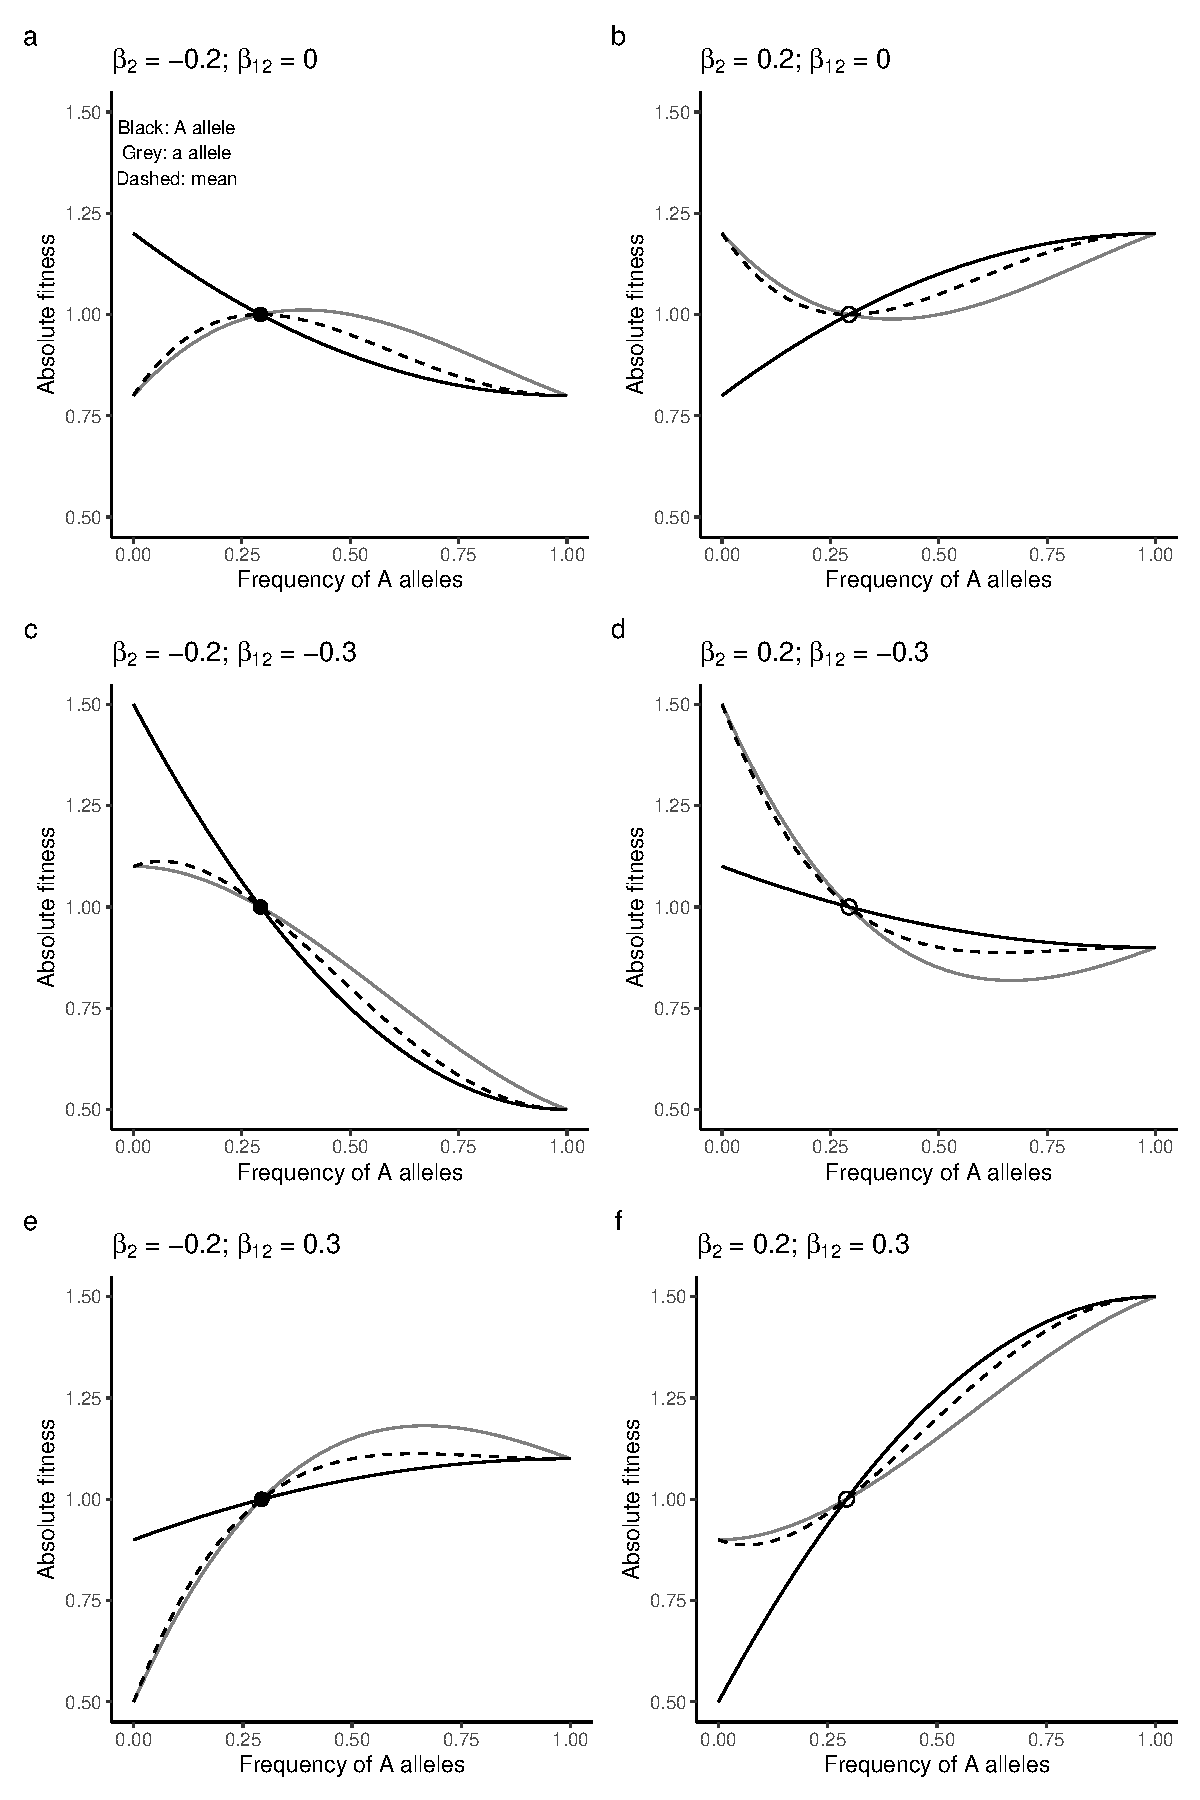
\includegraphics[width=0.95\linewidth]{AsymFDSdomi.pdf}
  \caption{Numerical examples for the fitness values $y_i$ in response to allele frequency when the A allele is completely dominant over the a allele. The black and gray lines indicate the allele-level fitness of A and a alleles; that is, Equations (\ref{eq:5a}) and (\ref{eq:5b}), respectively. Dashed curves indicate the population-level mean fitness  Equation (\ref{eq:6}). (a) Symmetric negative FDS, (d) symmetric positive FDS, (b and c) asymmetric negative FDS, and (e and f) asymmetric positive FDS. Closed and open circles indicate stable or unstable states, respectively. No directional selection i.e., $\beta_0=1.0$ and $\beta_1=0$ are assumed for all panels to present the fitness functions of FDS.}
  \label{fig2:asym}
\end{figure}


Population-level mean fitness under FDS is another side of interests when FDS concerns absolute fitness \citep{cockerham1972frequency,schneider_maximization_2008,takahashi2018balanced}. In a panmictic population, such a population-level mean fitness is given by the allele-level fitness weighted by its allele frequency (Appendix S2); that is, the weighted mean is given as follows:

\begin{equation}
\bar{y} = f y_\mathrm{A} + (1-f)y_\mathrm{a} = f^2 y_\mathrm{AA} + 2f (1-f)y_\mathrm{Aa} + (1-f)^2y_\mathrm{aa} \label{eq:6}
\end{equation}
\noindent
This population-level mean fitness is maximized at an intermediate frequency under symmetric negative FDS (Fig. \ref{fig2:asym}a) \citep{schneider_maximization_2008}. Even under an asymmetric negative FDS, the population-level mean fitness has a concave function against $f$ (Fig. \ref{fig2:asym}b and c), which indicates a larger population-level fitness than that expected by the frequency-independent selection \citep{takahashi2018balanced}. In contrast, the population-level mean fitness is minimized at an intermediate frequency under symmetric positive FDS (Fig. \ref{fig2:asym}d). Under the asymmetric positive FDS, the population-level mean fitness has a convex function (Fig. \ref{fig2:asym}e and f), and thus, it becomes less than expected by the frequency-independent selection \citep{schneider_maximization_2008, takahashi2018balanced}. When A and a alleles show additive expression as $x_i \in$ \{AA, Aa, aa\} $=$ \{+1, 0, -1\}, the fitness functions become so complicated that more than two equilibria may arise (Appendix S2; Fig. \ref{figS2:FDSadd}); however, they have rarely been reported empirically. Therefore, we assumed complete dominance for data analyses.

\subsection{Single-locus examples}
We determined whether the proposed regression models Equations (\ref{eq:2}) and (\ref{eq:3}) could detect negative FDS on single-locus dimorphism of hairy and glabrous phenotypes in a wild herb \textit{Arabidopsis halleri} (see "\textit{\textbf{Flower production of hairy and glabrous plants}}" below); and on single-locus polymorphism of female colors in a damselfly \textit{Ischnura elegans} (see "\textit{\textbf{Egg production of andromorph and gynomorph damselflies}}" below). These two systems from a plant and insect species share similar study designs. Both \textit{A. halleri} and \textit{I. elegans} cases involve absolute fitness values measured under the split subpopulation structure (Fig. \ref{fig1:scheme}a top). The fact that the trait expressions of both the trichome dimorphism and color polymorphism followed Mendelian inheritance with complete dominance \citep{shimizu2002ecology, sanchez2005hybridization, kawagoe2011coexistence} allowed us to substitute phenotype frequencies for the genotype frequencies of the heterozygote and dominant homozygote. These similar study designs from two different systems provided strong evidence for the rediscovery of negative FDS (see the results "\textbf{Single-locus examples}").

\subsubsection{Flower production of hairy and glabrous plants}
We applied single-locus analysis for the flower production data of \textit{Arabidopsis halleri} subsp. \textit{gemmifera} to detect negative FDS mediated by herbivore attacks on hairy and glabrous plants \citep{sato2017herbivore}. \cite{sato2017herbivore} recorded the trichome phenotype (hairy or glabrous), number of flowers, leaf damage score, and length of largest leaf for all individual plants after setting circular split plots (1 m in diameter) in a natural population at Japan (35$^\circ$06$^\prime$N, 134$^\circ$56$^\prime$E). Within these field plots, a flightless leaf beetle \textit{Phaedon brassicae} naturally occurred and fed on \textit{A. halleri} individuals. The total sample size comprised 3,070 individuals among 324 plots across four study years. Based on \cite{sato2017herbivore}, we used a generalized linear mixed model (GLMM) with a Poisson error structure and a log-link function to analyze the number of flowers as a countable response variable. The fixed effects were the individual phenotype (hairy or glabrous), similarity between the two morphs, and total number of plants within each field plot. While the total number of plants was implicitly incorporated as a denominator $N_k$ in Equations (\ref{eq:2}) and (\ref{eq:3}), this was also included as a fixed effect that represented plant density. Similar to that in \cite{sato2017herbivore}, the random effects were the field plot IDs nested below the study years. The log-transformed length of the largest leaf (mm), which reflects the plant size, was included as an offset term. In \textit{A. halleri}, hairy alleles are known to be dominant over glabrous alleles at the \textit{GLABRA1} locus \citep{shimizu2002ecology, kawagoe2011coexistence}. Given the complete dominance of hairy alleles, we assumed complete dominance at the \textit{GLABRA1} locus with $x_i \in$ \{AA, Aa, aa\} $=$ \{+1, +1, -1\} based on the trichome phenotype of an individual. The original data of \cite{sato2017herbivore} were downloaded from the Dryad repository (\url{https://doi.org/10.5061/dryad.53k2d}). The lme4 package \citep{bates2015} in R version 4.0.3 \citep{R_citation} was used for GLMM.

\subsubsection{Egg production of andromorph and gynomorph damselflies}
We applied the single-locus analysis for the egg production by the blue-tailed damselfly \textit{Ischnura elegans} to detect negative FDS and the consequent increase in population-level mean fitness between an andromorph and a gynomorph \citep{takahashi2014evolution}. The original data were derived from \cite{takahashi2014evolution} and consisted of 102 andromorphs and 79 \textit{infuscans}-type gynomorphs. \cite{takahashi2014evolution} assigned adult \textit{I. elegans} with an andromorph frequency of 0.2, 0.5, or 0.8 into split-field cages under low- or high-density conditions, and then counted the mature eggs. We used a GLMM with a Poisson error structure and a log-link function to analyze this countable response variable \cite{takahashi2014evolution}. The fixed effects were morph type and morph similarity within a cage. The cage ID and experimental ID were considered random effects, where the cage ID was nested below the experimental ID. The andromorph allele is known to be dominant over the \textit{infuscans}-type gynomorph allele on an autosomal locus \citep{sanchez2005hybridization}. Therefore, on the basis of phenotype frequencies within the split cages, we assumed complete dominance with genotype values encoded as $x_i \in$ \{AA, Aa, aa\} $=$ \{+1, +1, -1\} for homozygous andromorphs, heterozygous andromorphs, and homozygous gynomorphs, respectively. The interaction term between the morph type and similarity was considered in the line of GLMMs for testing the significance of asymmetric FDS between the two morphs. The coefficients of the main effect were estimated using GLMM without any interaction terms if it was not significant.

\subsection{GWAS extension}
We tested whether our method could aid in detecting FDS from genome-wide SNPs by extending the single-locus analysis to GWAS. We applied our regression methods for GWAS by implementing Equations (\ref{eq:2}) and (\ref{eq:3}) as linear mixed models (LMMs) that correct population genetic structure (see Appendix S3 "Mixed model extension"). To validate the performance of LMM implementation, we performed GWAS simulations under different selection regimes and subpopulation structures (see "\textit{\textbf{GWAS of simulated data}}" below). We also applied the extended GWAS method to empirical data on reproductive branch number in \textit{A. thaliana} accessions (see "\textit{\textbf{GWAS using field-grown Arabidopsis thaliana}}" below) to exemplify a GWAS-style experiment. This joint analysis using simulated and empirical data provides the first step to apply our method for a variety of GWAS data (see the results "\textbf{GWAS extension}").

\subsubsection{GWAS of simulated data}
We performed GWAS using simulated genomes and fitness values to test whether our regression method could distinguish FDS and other types of selection among genome-wide SNPs. In this simulation, we considered four scenarios of the selection process, which include negative FDS, positive FDS, overdominance, and spatiotemporally varying selection. Thirty independent rounds of three-step simulation ran as follows: (1) simulation of genomic structure under the four scenarios of selection, (2) virtual experiment to simulate fitness from the simulated genomes under the split or continuous subpopulation structure, and (3) fitting regression methods to simulated fitness and genomes. First, we used SLiM version 3 \citep{haller_slim_2019} to simulate SNPs for 2000 individuals (see Fig. \ref{figS4:GenStr} for the simulated genomic structure). We simulated the four scenarios of selection together with stabilizing selection on individual fitness to assume individual fitness as a quantitative trait. The simulated SNPs were imported to R using the vcfR \citep{knaus2017vcfr} and the gaston package \citep{R_gaston}. Second, we used the gaston \citep{R_gaston} and rNeighborGWAS \citep{sato2019neighbor} packages for fitness simulation. Out of the simulated individuals, 900 individuals are randomly assigned to split (Fig. \ref{fig1:scheme}a top) or continuous (Fig. \ref{fig1:scheme}a bottom) subpopulations. We simulated fitness values based simulated SNPs with the ratio of genetic variance on non-genetic variance kept at two third. Third, simulated fitness values were fitted using the LMM version of Equation (\ref{eq:2}) (Appendix S3), which estimated the genotype similarity effect $\hat{\beta}_2$ and its -log\textsubscript{10}($p$-values) association score for all SNPs. For the fitness simulation and fitting, we focused on the symmetric FDS on relative fitness because the selection acted not on absolute but on relative fitness during the SLiM simulation above. We used the receiver operating characteristic (ROC) curve implemented in the pROC \citep{R_pROC} package to quantify the false vs. true positive rate of causal SNP detection by the -log\textsubscript{10}($p$-values) association score. The model performance was evaluated by the area under the ROC curve (AUC). We performed the line of simulations using both LMs and LMMs to test the notion that linear mixed models (LMMs) usually outperform standard linear models (LMs) in GWAS \citep{kang2008efficient}. Further, to examine the influence of heterozygosity on the model performance, we tested additive and dominant genotype encoding in the line of simulations. The details of these GWAS simulations are provided in Appendix S4.

\subsubsection{GWAS using field-grown \textit{Arabidopsis thaliana}}
We conducted a pilot GWAS of the reproductive branch number in field-grown \textit{A. thaliana} under a continuous setting to examine whether our method is applicable to the empirical GWAS dataset (Fig. \ref{fig1:scheme}a bottom). We first set three randomized blocks of 199 \textit{A. thaliana} accessions in a field site at Zurich, Switzerland to observe the final reproduction. The experimental procedure followed that of \cite{sato2019neighbor}, with slightly modifications for the present study (see Appendix S5 for details). From early summer (July 8, 2019), we recorded the length of the largest leaf (mm) at the beginning of the experiment, the presence of bolting after 2 weeks, and the reproductive branch number at the end of the experiment (August 27, 2019). Further, we quantified a reproductive fitness component by the number of reproductive branches that had at least one trace of flowers because it was difficult to assess the exact number of flowers for diverse accessions under the harsh summer environment. Dead plants were recorded as a branch number of zero, \textit{ i.e. }, with no fecundity. The number of reproductive branches was log(x+1)-transformed to improve normality, and it was analyzed as a target trait of GWAS. With the cut-off threshold of minor allele frequency at >0.05, we obtained 1,819,577 SNPs from genotype data registered in the AraGWAS catalog \citep{togninalli_aragwas_2018}. The inbred lines of \textit{A. thaliana} have either the AA or aa genotype, in which the qualitative interpretation of $\beta_2$ and $\beta_{12}$ in this inbred case remains the same as in the case of complete dominance (Appendix S2; Fig. \ref{figS3:FDSinbred}). We assumed that FDS arose from genetic interactions among neighboring plants in small \textit{Arabidopsis}, and therefore, the genotype similarity was considered up to the nearest neighbors. The initial plant size, presence of bolting, experimental block ID, and edge of each plot (or not) were considered as nongenetic covariates. The rNeighborGWAS package version 1.2.4 \citep{sato2019neighbor} was used to implement Equations (\ref{eq:2}) and (\ref{eq:3}) as GWAS (Appendix S3). After association mapping, we focused on SNPs with a -log\textsubscript{10}($p$-value) score $>$ 4.0. We searched candidate genes within $\sim$10 kb around the target SNPs based on the Araport11 gene model with the annotation of The Arabidopsis Information Resource (TAIR; accessed on 31 December 2021). Accession names and phenotype data are presented in Table \ref{tableS3:GWASdata}. The details of the field GWAS experiment are provided in Appendix S5.

\section{Results}

\subsection{Single-locus examples}

\begin{figure}[ht]
  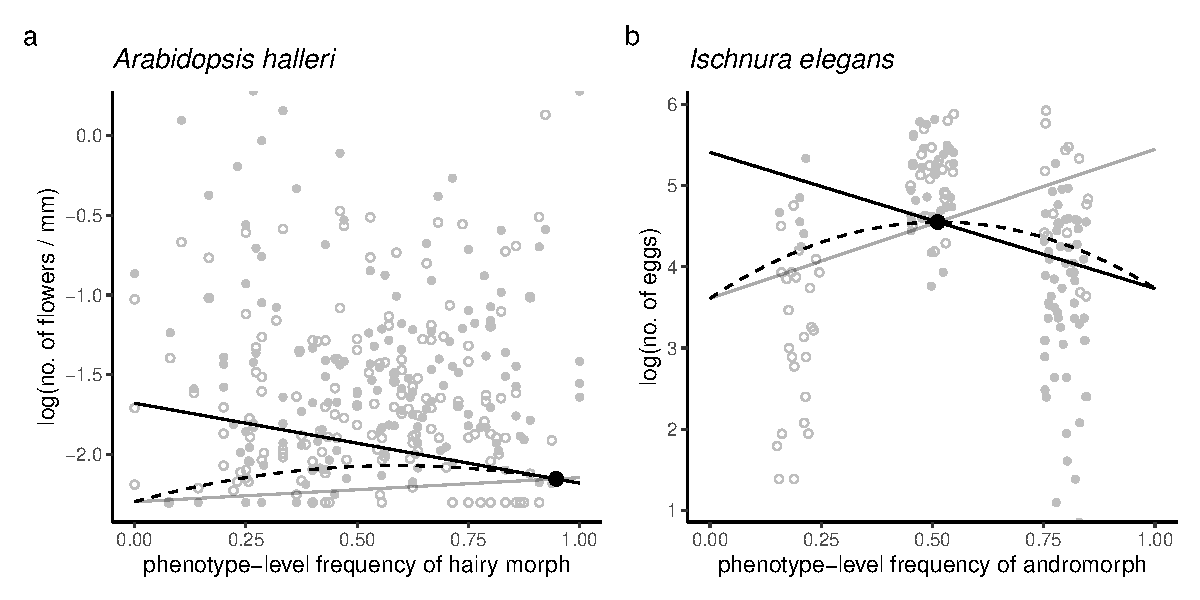
\includegraphics[width=0.9\linewidth]{Ah_Ie_plots.pdf}
  \caption{Negative frequency-dependent selection on (a) the flower production of hairy and glabrous plants in \textit{A. halleri} and (b) the egg production of andromorph and gynomorph females in \textit{I. elegans}. Estimated fitness function based on the fitted model (Table \ref{table1:GLMM}) are shown at a phenotype level (see case 3 in Appendix S2). Gray circles and the solid black line indicate observed and predicted fitness of dominant morphs (i.e., hairy and andromorph), respectively, while the white open circles and solid gray line indicate those of recessive morphs (glabrous and gynomorph), respectively. The dashed curve presents the population-level mean fitness based on the fitted model (Table \ref{table1:GLMM}), with a black dot indicating the stable equilibrium under negative FDS. A single circle in panel (a) corresponds to a field plot, where the flower production represents the plot-level average of log[(no. of flowers / plant size (mm)) + 0.1]. A single circle in panel (b) corresponds to an individual morph, where the egg production represents log(no. of mature eggs).}
  \label{fig3:GLMM}
\end{figure}

\subsubsection{Negative FDS on trichome dimorphism in a wild \textit{Arabidopsis}}
We applied Poisson GLMM for the flower production data on hairy and glabrous plants of \textit{A. halleri} within split field plots (see the methods "\textit{\textbf{Flower production of hairy and glabrous plants}}" above) to test whether the single-locus analysis could detect the known negative FDS. The Poisson GLMM detected a negative and significant coefficient of the morph similarity $\hat{\beta}_2$ (Table \ref{table1:GLMM}a), which indicates a negative FDS where a focal plant produced more flowers as dissimilar morphs were grown within the same plot. This negative FDS was symmetric between hairy and glabrous plants, as indicated by the lack of significance of the interaction term between the trichomes and morph similarity (Table \ref{table1:GLMM}a). Further, we found the same level of the individual morph coefficient $\hat{\beta}_1$ as the negative coefficient of morph similarity $\hat{\beta}_2$ (Table \ref{table1:GLMM}a); this indicates the simultaneous action of directional selection and negative FDS between the two morphs. The flower production was not dependent on the plant density as indicated by no significant effects from the total number of plants (Table \ref{table1:GLMM}a). The estimated fitness function based on the fitted model (Table \ref{table1:GLMM}) show that a stable equilibrium under negative FDS remains at a biased but not monomorphic frequency (Fig. \ref{fig3:GLMM}a). This discrepancy between the observed frequency and expected equilibrium was likely because the present selection analysis could not incorporate another major component of fitness in \textit{A. halleri}; i.e., clonal reproduction \citep{sato2017herbivore}. These results provide qualitative evidence for negative FDS on trichome dimorphism through the fitness component of flower production.

\begin{table}[ht]
\caption{Poisson generalized linear mixed model (GLMM) applied to the number of flowers between hairy and glabrous \textit{A. halleri} (a) or the number of mature eggs between the andromorph and gynomorph of \textit{I. elegans} (b). Morph similarity was calculated from the genotype similarity defined by Equation (\ref{eq:2}). Estimated coefficients, their standard errors (SE), $Z$-values, and $p$-values are shown for multiple regressions. Bold letters indicate significance at $p <$ 0.05 by Wald tests.}
(a) \textit{Arabidopsis halleri} \\
\begin{tabular}{lllll}
\hline
\multicolumn{1}{c}{Fixed effects} & \multicolumn{1}{c}{Coefficient} & \multicolumn{1}{c}{SE} & \multicolumn{1}{c}{\textit{Z}} & \multicolumn{1}{c}{\textit{p}} \\ \hline
\textbf{Intercept} $\hat{\beta}_{0}$    & \textbf{-2.076}  &  \textbf{0.17} & \textbf{-11.97} & \textbf{\textless{}2e-16}  \\
\textbf{Individual morph} $\hat{\beta}_{1}$      & \textbf{0.146}                  & \textbf{0.008}         & \textbf{17.32}                 & \textbf{\textless{}2e-16}      \\
\textbf{Morph similarity} $\hat{\beta}_{2}$        & \textbf{-0.163}                 & \textbf{0.018}         & \textbf{-9.22}                 & \textbf{\textless{}2e-16}      \\
Total no. of plants               & -0.006                          & 0.010                  & -0.63                          & 0.53                           \\
Self $\times$ Similarity $\hat{\beta}_{12}$            & -0.088                          & 0.048                  & -1.81                          & 0.07                           \\ \hline
\end{tabular}

\vspace*{5mm}

(b) \textit{Ischnura elegans} \\
\begin{tabular}{lllll}
\hline
\multicolumn{1}{c}{Fixed effects} & \multicolumn{1}{c}{Coefficient} & \multicolumn{1}{c}{SE} & \multicolumn{1}{c}{\textit{Z}} & \multicolumn{1}{c}{\textit{p}} \\ \hline
\textbf{Intercept} $\hat{\beta}_{0}$    & \textbf{4.55} &  \textbf{0.191} & \textbf{23.8}  & \textbf{\textless{}2e-16}  \\
\textbf{Individual morph} $\hat{\beta}_{1}$               & \textbf{-0.021}                 & \textbf{0.008}         & \textbf{-2.56}                 & \textbf{0.01}                  \\
\textbf{Morph similarity} $\hat{\beta}_{2}$           & \textbf{-0.878}                 & \textbf{0.022}         & \textbf{-39.30}                & \textbf{\textless{}2e-16}      \\
Density                             & 0.097                           & 0.237                  & 0.41                           & 0.68                           \\
Self $\times$ Similarity $\hat{\beta}_{12}$                 & -0.042                          & 0.25                 & -0.17                          & 0.87                           \\ \hline
\end{tabular}
\label{table1:GLMM}
\end{table}

\subsubsection{Negative FDS on female color polymorphisms in a damselfly}
To test whether the single-locus analysis could detect a known relationship between negative FDS and population-level mean fitness, we applied Poisson GLMM for the data on the number of mature eggs between the andromorph and gynomorph of \textit{I. elegans} within split field cages (see the methods "\textit{\textbf{Egg production of andromorph and gynomorph damselflies}}" above). Consistent with the previous evidence for negative FDS \citep{van2001frequency, le2015evolutionary}, we found a significantly negative coefficient of morph similarity $\hat{\beta}_2$ (Table \ref{table1:GLMM}b). The interaction term between the morph type and similarity was not significant (Table \ref{table1:GLMM}b), indicating no significant asymmetry in the negative FDS between the two morphs. We also found a significant effect of the morph type (andromorph or gynomorph) on the egg production, but its effect was much less significant than that of morph similarity (Table \ref{table1:GLMM}b). As reported in a previous study \citep{takahashi2014evolution}, the density did not significantly affect the egg production (Table \ref{table1:GLMM}b). Estimated fitness function based on the fitted model (Table \ref{table1:GLMM}) shows that the negative FDS enabled the coexistence of the two morphs at an intermediate frequency (Fig. \ref{fig3:GLMM}b). Consistent with the results of \cite{takahashi2014evolution}, the population-level mean fitness increased at a stable equilibrium at the intermediate frequency under the negative FDS (Fig. \ref{fig3:GLMM}b). These results support the action of symmetric negative FDS and the consequent increase in the population-level mean fitness. Taken together, \textit{A. halleri} and \textit{I. elegans} data suggest that our single-locus model can be applied to the selection gradient analyses of FDS (see also the discussion "\textbf{Selection gradient along genotype similarity}").

\subsection{GWAS extension}

\subsubsection{Detection of simulated FDS across a genome}
We simulated genotypes and fitness to test whether our method could distinguish negative FDS, positive FDS, overdominance, and spatiotemporally varying selection among genome-wide SNPs (see the methods "\textit{\textbf{GWAS of simulated data}}" above; Appendix S4; and Figs. \ref{figS5:beta2LM}-\ref{figS:beta2LMadd}). We further implemented the single-locus model Equation (\ref{eq:2}) as a linear mixed model (LMM) (Appendix S3) to correct the population genetic structure in GWAS. Assuming the complete dominance of A over a alleles, we first evaluated the performance of these LMMs in terms of causal polymorphism detection and effect size estimates (Fig. \ref{fig4:beta2LMM}). The performance of LMMs to detect negative and positive FDS was high in both split and continuous settings (median performance $>0.8$; Fig. \ref{fig4:beta2LMM}b and e). The direction of the FDS matches the estimated sign of $\beta_2$ (Fig. \ref{fig4:beta2LMM}c and f). In contrast, these LMMs showed little or weak performance to detect overdominance or spatiotemporally varying selection, respectively (median performance $< 0.6$; Fig. \ref{fig4:beta2LMM}b and e), and their estimated coefficients were almost zero (Fig. \ref{fig4:beta2LMM}c and f). Further, we tested another general assumption of GWAS, i.e., the additive effects of two allele on fitness, which resulted in the moderate to high performance of LMMs in detecting negative and positive FDS (Fig. \ref{figS:beta2LMMadd}; Appendix S4). These results indicate that our method retains the statistical power to detect negative and positive FDS in GWAS, with other types of balancing selection less likely to be confounded. 

\begin{figure}[ht]
  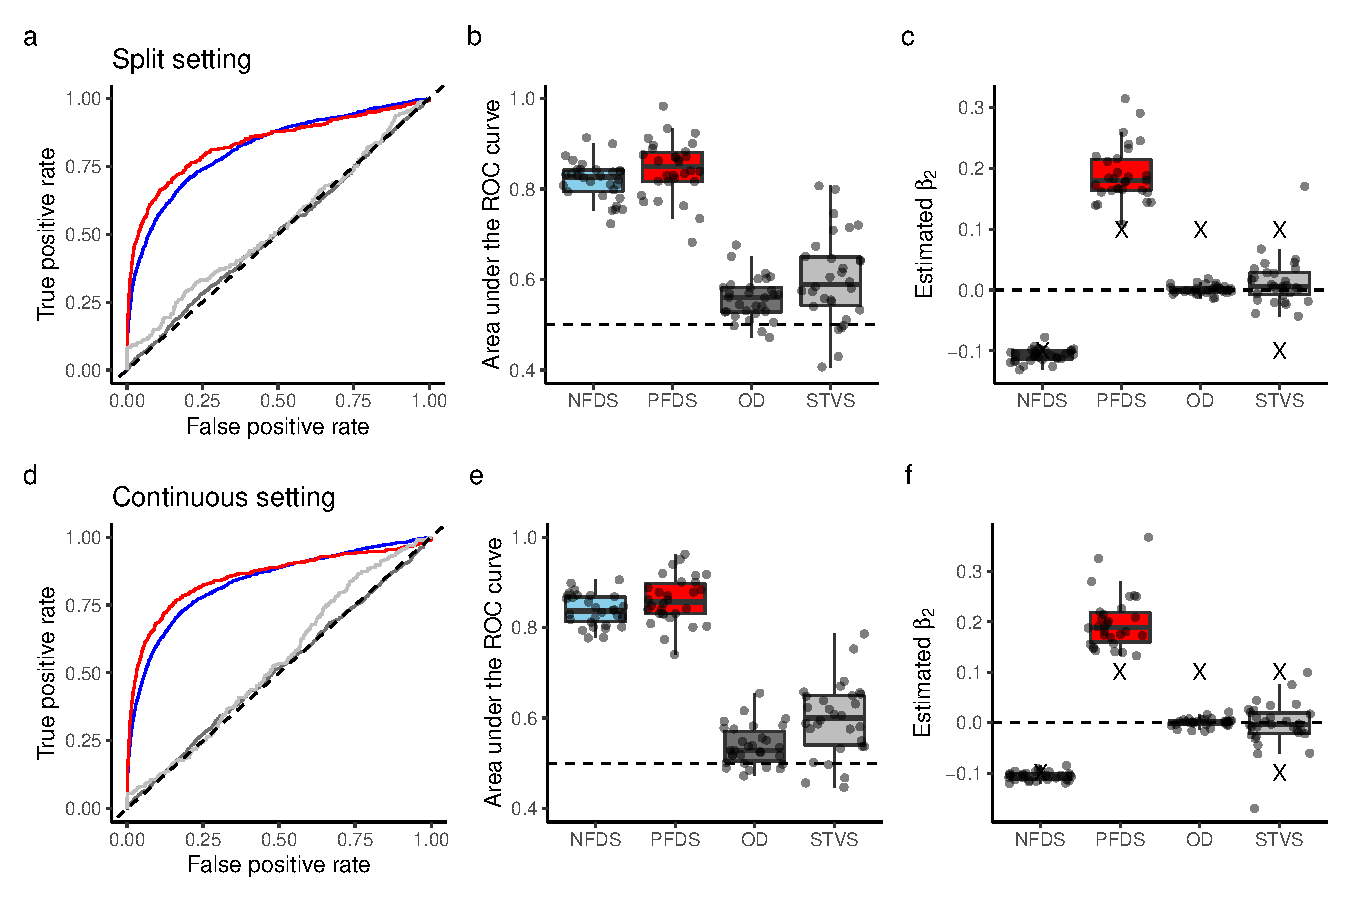
\includegraphics[width=0.85\linewidth]{beta2LMMdomi.pdf}
  \caption{Performance of linear mixed models for detecting four types of simulated selection among genome-wide polymorphisms: NFDS, negative frequency-dependent selection (blue); PFDS, positive frequency-dependent selection (red); OD, overdominance (dark gray); and STVS, spatiotemporally varying selection (light gray). The top and bottom panels show the results of the split and continuous settings of subpopulation structure, respectively (Fig. \ref{fig1:scheme}a). (a and d) The receiver operating characteristic (ROC) curve showing the relationships between the true and false positive rates. (b and e) Model performance evaluated by the area under the ROC curve (AUC). Dashed lines at 0.5 indicate no statistical power to detect causal single nucleotide polymorphisms (SNPs). (c and f) Estimated $\beta_2$ of causal SNPs, where the negative and positive values indicate negative and positive FDS, respectively. Cross marks indicate the true simulated magnitude of $\beta_2$. Boxplots show the median by a center line, upper and lower quartiles by box limits, and 1.5$\times$ interquartile range by whiskers.}
  \label{fig4:beta2LMM}
\end{figure}

Then, we compared the performance of LMMs with that of standard LMs to inspect whether the correction of population genetic structure improved GWAS (Fig. \ref{fig4:beta2LMM}, Fig. \ref{figS5:beta2LM}; Appendix S4). LMMs better detected negative FDS than LMs in terms of the model performance (Fig. \ref{fig4:beta2LMM}b and e, Fig. \ref{figS5:beta2LM}b and e). Although LMs and LMMs exhibited similar performances for positive FDS, the LMs overestimated the true strength of positive FDS more than LMMs (Fig. \ref{fig4:beta2LMM}c and f, Fig. \ref{figS5:beta2LM}c and f). Even when we assumed additive fitness effects from two alleles, the LMMs better detected negative FDS and less overestimated positive FDS than that with LMs (Fig. \ref{figS:beta2LMMadd} and Fig. \ref{figS:beta2LMadd}; Appendix S4). These results suggest that LMMs are better suited to the proposed method because they can more efficiently capture negative FDS or prevent overestimation of the strength of positive FDS.

\subsubsection{Patterns of FDS in the \textit{Arabidopsis thaliana} genome}
We applied an LMM for the GWAS of the reproductive branch number in \textit{A. thaliana} (Fig. \ref{fig5:gwas}) under the continuous setting (Fig. \ref{fig1:scheme}a bottom) to demonstrate feasibility using an empirical GWAS dataset (see the methods "\textit{\textbf{GWAS using field-grown Arabidopsis thaliana}}" above; Appendix S5; and Figs. \ref{figS9:QQplotLMM}-\ref{figS11:QQplotLM}). To diagnose our data, we examined the individual genotype effects $\beta_1$ using a standard GWAS. The association mapping of the individual genotype effects $\beta_1$ detected no significant SNPs above the Bonferroni threshold; however, a weak peak was observed on the top of chromosome 4 (Fig. \ref{fig5:gwas}a; Table \ref{tableS4:GWAScandidates}a; see also Fig. \ref{figS9:QQplotLMM} for quantile-quantile plots). The top of chromosome 4 is known to encompass a flowering QTL near the \textit{FRIGIDA} gene \citep{atwell2010genome}. Our results of individual genotype effects agree with previous evidence and support the usefulness of our GWAS data.

To examine the relevance of symmetric FDS, we next tested the significance of the genotype similarity effects $\beta_2$ for all SNPs. To elucidate the genome-wide patterns of $\beta_2$ and candidate genes, we focused on SNPs exhibiting $p$-values of $<$ $10^{-4}$. Of the 254 SNPs selected, 195 and 59 showed negative and positive $\beta_2$, respectively (Fig. \ref{fig5:gwas}d), which indicates the prevalence of negative FDS in the \textit{A. thaliana} genome. This excess of negative $\hat{\beta}_2$ was consistently observed even when we used LMs (Fig. \ref{figS10:gwasLM}d). To obtain a functional inference, we focused on candidate genes near top-scoring SNPs. Within 10 kbp near the top-scoring SNP on chromosome 3 (Fig. \ref{fig5:gwas}b), we observed the \textit{GAE6} gene, which encodes a UDP-D-glucuronate 4-epimerase involved in pectin biosynthesis, cell wall integrity, and immunity to pathogens \citep{bethke2016pectin}. Genes involved in plant immunity and resistance, such as \textit{GAE6}, \textit{ARGONAUTE 4} (\textit{AGO4}), and \textit{ACTIVATED DISEASE RESISTANCE 1} (\textit{ADR1}), were observed within 10 kb near the SNPs showing negative $\beta_2$ at $p$-value $< 10^{-4}$ (Table \ref{tableS4:GWAScandidates}b). In contrast, \textit{AVRRPT2-INDUCED GENE 1} (\textit{AIG1}) was only a resistance-related gene observed near the SNPs showing positive $\hat{\beta}_2$ at $p$-values of $< 10^{-4}$ (Table \ref{tableS4:GWAScandidates}b); these results suggest the potential relevance of disease resistance genes to the widespread pattern of negative FDS.

\begin{figure}[ht]
  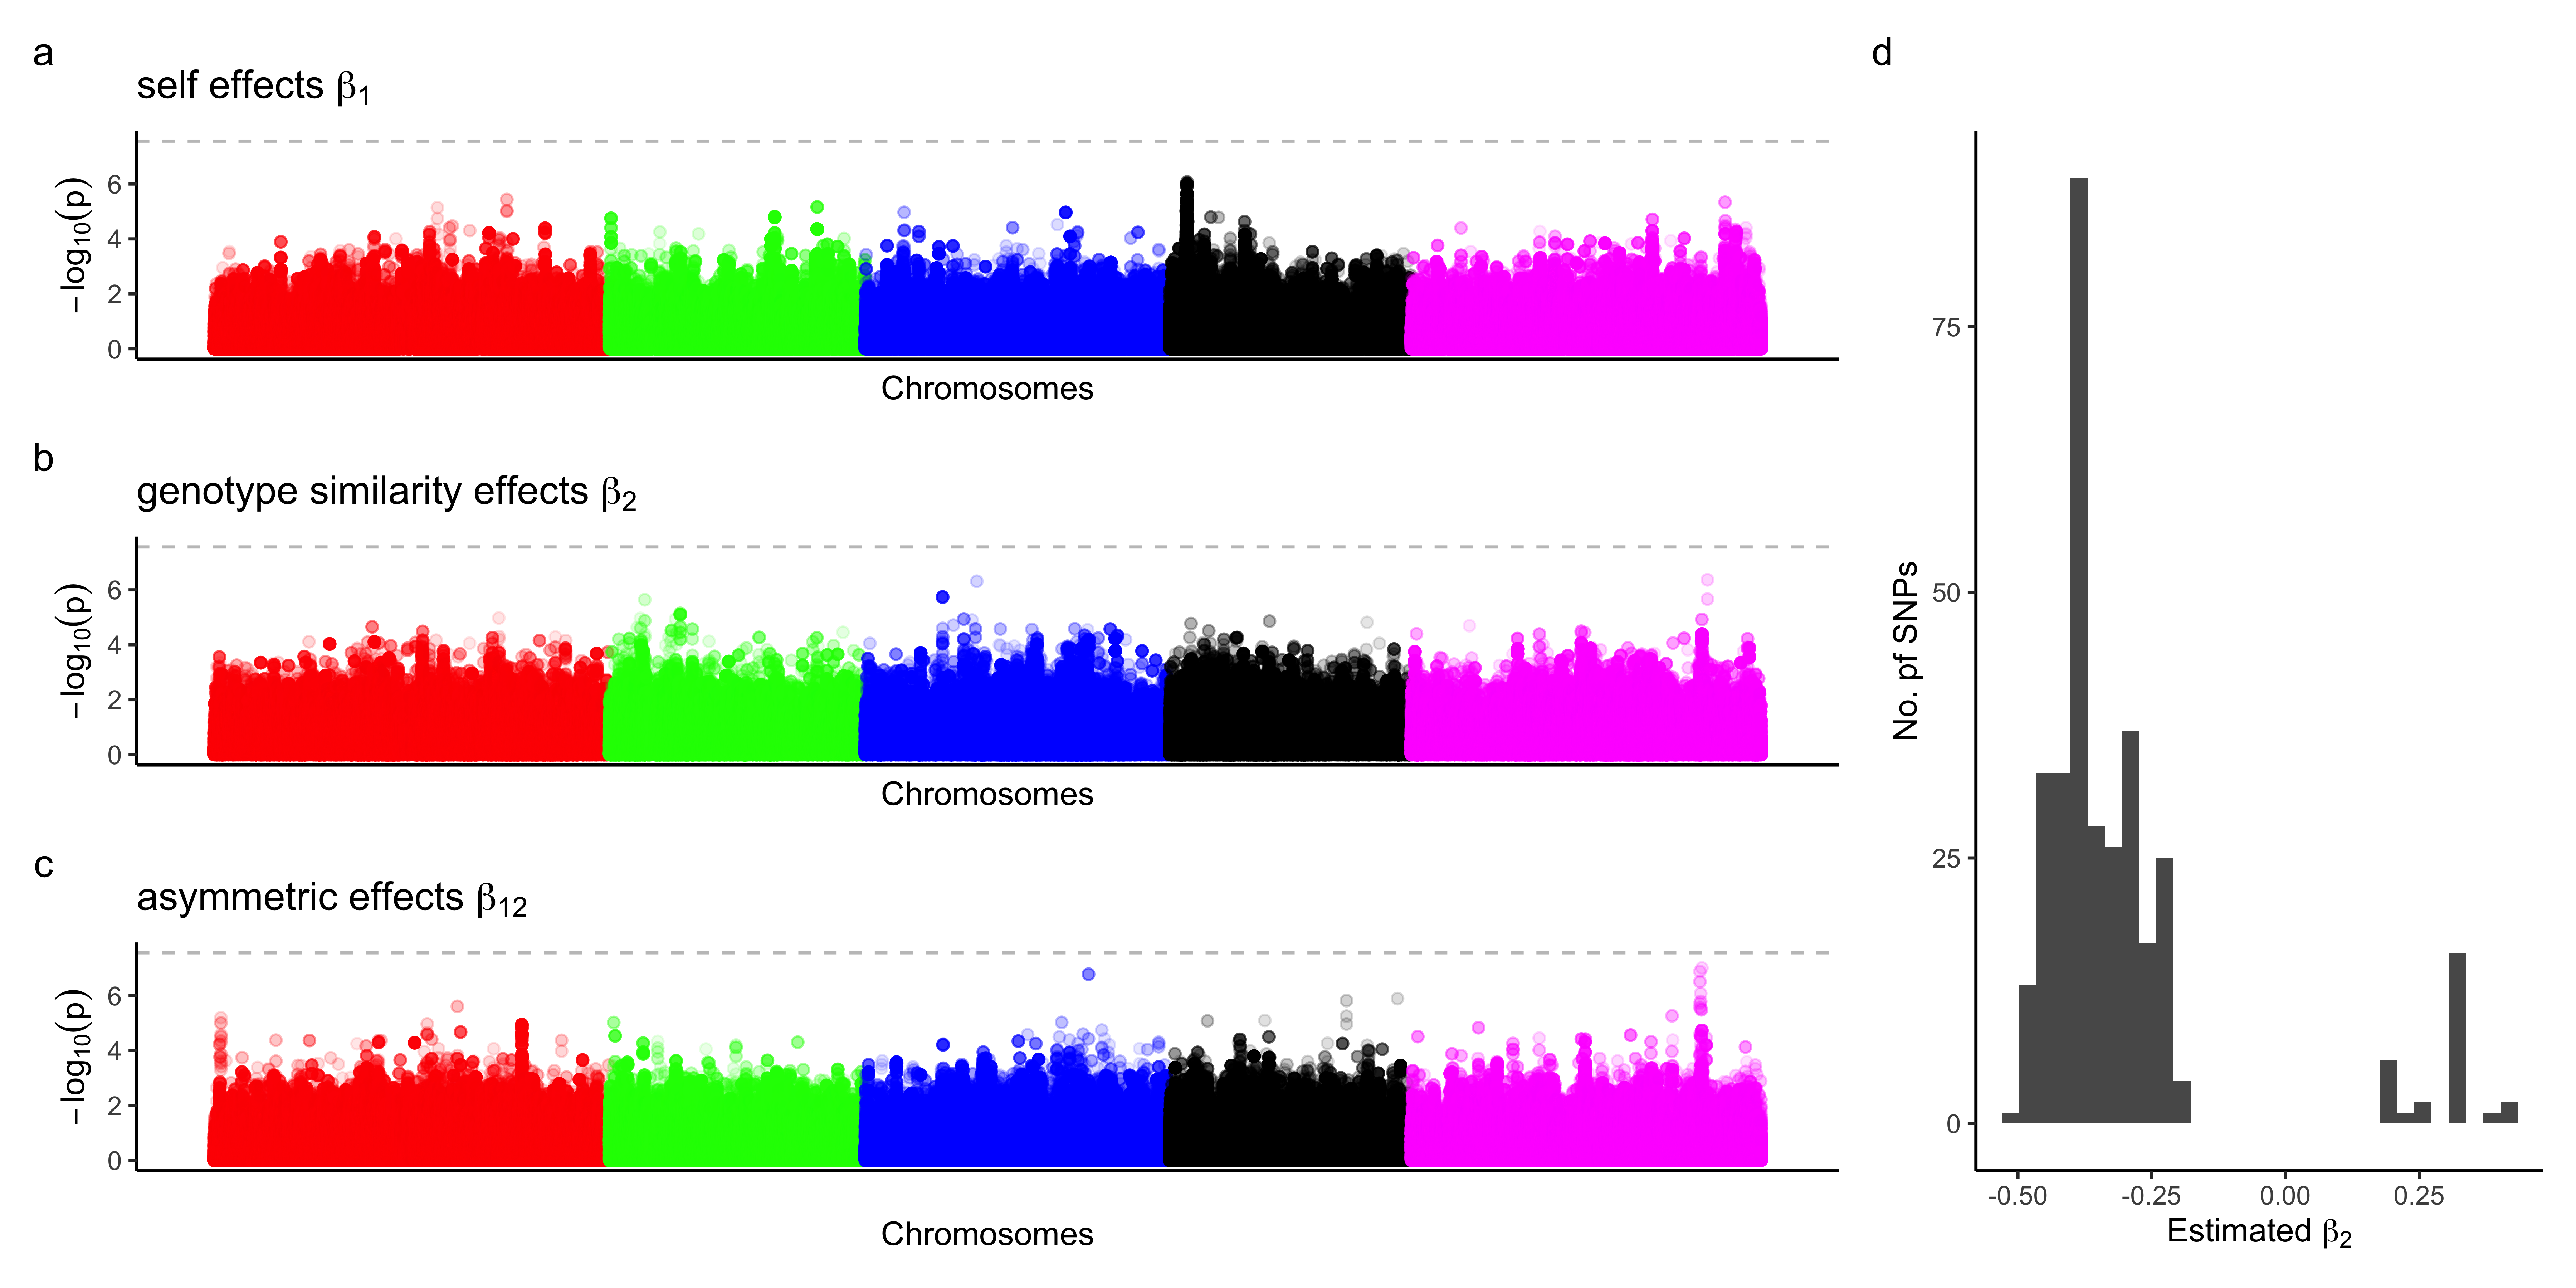
\includegraphics[width=\linewidth]{ManhattanLMM.png}
  \caption{Genome-wide association studies of reproductive branch number in field-grown \textit{Arabidopsis thaliana} under the continuous population setting (Fig. \ref{fig1:scheme}a bottom). The results of linear mixed models are shown. (a, b, and c) Manhattan plots showing the association score of -log\textsubscript{10}($p$-values) for individual genotype effects, genotype similarity effects, and asymmetric effects, respectively. Horizontal dashed lines indicate $p$-value $=$ 0.05, after Bonferroni correction. (d) The histogram of estimated $\beta_2$ among SNPs exhibiting $p$-values $< 10^{-4}$. The negative and positive $\beta_2$ infer loci responsible for negative and positive FDS, respectively.}
  \label{fig5:gwas}
\end{figure}

We then tested the asymmetric effects $\beta_{12}$ for all SNPs to examine the relevance of asymmetric FDS. We detected a QTL on chromosome 5 near the Bonferroni threshold (Fig. \ref{fig5:gwas}c). These SNPs exhibited positive $\beta_2$ and $\beta_{12}$ (i.e., $\hat{\beta}_2=0.78$ and $\hat{\beta}_{12}=1.13$ on chromosome 5 at position 22382673: Table \ref{tableS4:GWAScandidates}c), indicating positive effects of a reference allele on absolute fitness together with positive FDS on relative fitness. Genes potentially related to growth were located near this top-scoring SNP, including \textit{SUMO2} and \textit{SUMO3}. In the line of GWAS analyses, the individual genotype effect $\beta_1$, symmetric FDS $\beta_2$, and asymmetric $\beta_{12}$ did not share any SNPs that exhibited $p< 10^{-4}$. The sort of top-scoring SNPs and candidate genes infer different functions among individual genotype effects, symmetric negative FDS, and asymmetric positive FDS.

We examined a potential bias of -log\textsubscript{10}($p$-values) association scores based on quantile-quantile plots (Fig. \ref{figS9:QQplotLMM} and Fig. \ref{figS11:QQplotLM}) to inspect whether LMMs yields better results than LMs. Quantile-quantile plots of LMMs exhibited a slight inflation of the observed association score against the expected score for the genotype similarity effects $\beta_2$ and asymmetric effects $\beta_{12}$ (Fig. \ref{figS9:QQplotLMM}b-c), whereas those of LMs showed slightly inflated scores (Fig. \ref{figS11:QQplotLM}b-c). Combined with the simulation above, these empirical results suggest that LMMs are more suitable for GWAS than LMs. The line of GWAS simulation and application suggests that our method can also be used to screen polymorphisms associated with FDS (see also the discussion "\textbf{Applicability for GWAS}").

\section{Discussion}

\subsection{Selection gradient along genotype similarity}
Selection gradient analysis is a powerful approach for empirical studies to quantify selection in action \citep{lande1983measurement, mitchell1987regression, chong2018note}. The incorporation of population-level covariates offers further opportunity to reveal how selection depends on population contexts \citep{heisler1987method}. To analyze FDS, empirical studies have often incorporated morph frequency such as the population-level covariate and regressed fitness components on the morph frequency \citep{gigord2001negative, mccauley1998frequency, calsbeek2010geographic, sato2017herbivore}. We propose a simple regression model where the two regression coefficients $\beta_2$ and $\beta_{12}$ represent FDS on relative and absolute fitness, respectively, by incorporating genotype similarity as a covariate. As the covariate of genotype similarity $(\sum^{N_k}_{j=1}x_i x_j)/N_k$ denotes how similar (or dissimilar) the neighbor compositions are with the focal individual, conclusions are expected to be the same as we regress fitness components on the frequency of other morphs. In fact, the single-locus analysis detected known negative FDS in \textit{A. halleri} and \textit{I. elegans}, and it was attributed to the negative sign of $\beta_2$. These reanalyses exemplify the simple and wide usability of our regression model for plants and animals in natural or semi-natural fields. 

The population-level mean fitness is another side of interests in a general model of FDS when FDS acts on absolute fitness \citep{cockerham1972frequency,asmussen_frequency-dependent_1990,schneider_maximization_2008}. Based on the regression model of FDS, our method provides an additional inference of the relationships between the population-level mean fitness and allele frequency (Fig. \ref{fig2:asym}). For example, symmetric negative FDS lead the population-level mean fitness to increase at an intermediate allele frequency (Fig. \ref{fig2:asym}a). Empirical studies on \textit{I. elegans} reported such an increased population-level mean fitness at an intermediate frequency \citep{takahashi2014evolution} as well as negative FDS on female color polymorphisms \citep{le2015evolutionary}. This previous evidence is supported by our reanalysis showing symmetric negative FDS (i.e., $\hat{\beta}_2<0$; Table \ref{table1:GLMM}b) and a consequent increase in population-level mean fitness at an intermediate frequency in \textit{I. elegans} (Fig. \ref{fig3:GLMM}b). Although the reanalysis of \textit{A. halleri} data shows the biased frequency on its equilibrium, negative FDS still maintained the dimorphism and very slightly increased population-level mean fitness at the equilibrium frequency (Fig. \ref{fig3:GLMM}a). In addition to the efficient detection of FDS, the present method provides an empirical approach to understand how FDS increases population-level mean fitness.

\subsection{Applicability for GWAS}
Selection gradient analysis is used for genome-wide studies to quantify the ongoing selection \citep[e.g.,][]{exposito2019natural, groen2020strength}. We extended our regression method to LMMs that have often been used in GWAS by incorporating the population genetic structure as random effects \citep[e.g.,][see also Appendix S3]{kang2008efficient, gondro2013genome}. Our simulations suggest that LMMs improve the statistical power to detect causal polymorphisms or prevent us from exaggerating effect-size estimates of FDS. We should also focus on the genetic structure of loci underlying positive or negative FDS to correctly understand the power of LMMs. Because positive FDS reduces polymorphisms, their selected loci likely showed low heterozygosity and strong population differentiation (Fig. \ref{figS4:GenStr}). Although LMMs can deal with the population genetic structure to some extent, their effect-size estimates are still larger than the true signals (Fig. \ref{fig4:beta2LMM}c and f). This seems consistent with the general notion that a systematic bias, such as the incomplete correction of population genetic structure, leads GWAS to inflate association estimates \citep{gondro2013genome}. The overestimation of positive FDS may thus be because of a strong correlation in the genetic structure between neutral and selected loci under positive FDS. In contrast, negative FDS results in high heterozygosity by maintaining polymorphisms within a population (Fig. \ref{figS4:GenStr}) where LMMs can perform better than LMs by separating the neutral genetic structure and loci subject to negative FDS. While the current application is limited to homozygous \textit{A. thaliana}, our simulations clarified what should be considered to analyze heterozygous individuals.

The application to \textit{A. thaliana} accessions found a genome-wide excess of negative FDS and a few loci underlying asymmetric positive FDS. This result seems plausible because polymorphic loci are more likely to persist under negative FDS than positive FDS. In the present study, we found candidate genes that might be involved in conferring plant resistance to pathogens. This finding supports the hypothesis that negative FDS is likely to act on the polymorphism of pathogen resistance \citep{antonovics1984experimental, brunet2000disease}. In contrast, such resistance genes were not found near the loci responsible for asymmetric positive FDS. We instead found growth-related candidate genes near the loci associated with asymmetric positive FDS. The asymmetric and positive frequency-dependent effects from tall to short plants is known to occur in plant competition \citep{weiner1990asymmetric}, where growth-related loci are more likely to be observed than defense-related loci. However, our field experiment provides a one-year snapshot of FDS in a common garden, and it does not indicate the long-term importance of FDS compared to other selective pressures responsible for genomic variation among \textit{A. thaliana} accessions. These accessions were originally collected from different natural populations \citep{horton_genome-wide_2012, alonso-blanco_1135_2016}, and thus, the extent to which the common garden experiment simulates naturally co-occurring alleles is also elusive. Further, the branch number remains a qualitative measure that presumably has a strong association with fitness in \textit{A. thaliana} \citep{chong2018note}. Further studies using an accurate fitness data in varying space and time will be required to verify the patterns of FDS in the \textit{A. thaliana} genome. Limited datasets are currently available to reveal general patterns of FDS because our methods require exact spatial positions or subpopulation structure for individuals. If open data are registered with the spatial positions as well as individual genotypes and fitness, these datasets suit the analysis of FDS using our method.

\subsection{Potential limitation}
In addition to the model of one locus with two alleles \citep{cockerham1972frequency, asmussen_frequency-dependent_1990, schneider_maximization_2008}, FDS have been theoretically analyzed in relation to one locus with multi-alleles \citep{schneider2006multilocus, trotter2007frequency} and multi-loci with multiple alleles \citep{schneider2010maximization}. Even a one-locus two-allele model can make fitness functions have multiple equilibria when it involves the additive action of FDS on a quantitative trait \citep[][Fig. \ref{figS2:FDSadd}; Appendix S2]{schneider_maximization_2008}; however, more complex outcomes are possible in the realistic genetic architecture. Since our method is customized to detect simple instances of FDS, other more complicated actions of FDS are unlikely to be captured by the proposed regression model. For example, FDS can act on more than two co-dominant alleles at a single locus, such as the S-allele system in plant self-incompatibility \citep{hatakeyama1998dominance, shimizu2015evolution}. The multi-allele extension of our regression model would be required to widen its applicability for the well-reported instances of FDS. 

\subsection{Conclusion}
This study offers an effective method to model the patterns of fitness-genotype associations with respect to FDS. Our phenotype-driven approach can distinguish between positive and negative FDS based on the direct observations of fitness components. Although considerable effort is required to measure individual fitness, a selection gradient analysis has an advantage in quantifying ongoing FDS. Such a snapshot of the ongoing selection may not always match the past signatures of selection; however, a joint study using the genomic signature and selection gradient analysis will reveal consistent patterns of FDS throughout the genome. In molecular population genetics, phenotype-free methods are available for detecting the signatures of past balancing selection \citep{siewert_detecting_2017}. Now that genome information is accumulating in wild organisms \citep{lewin2018earth}, organismal biologists may utilize genome data for a deeper understanding of the maintenance of polymorphism from the past to present. Our pilot test using \textit{A. thaliana} accessions is expected to provide the first step to reveal genome-wide patterns of FDS in the field.

\section*{Data Availability Statement}
The source codes and original data generated by this study are available in the GitHub repository (\url{https://github.com/yassato/RegressionFDS}) and its published version is deposited on Dryad (\url{https://doi.org/10.5061/dryad.zs7h44jdv}). A vignette using toy data is available at \url{https://yassato.github.io/RegressionFDS}, and its source files are included in the GitHub and the Dryad repository.

\section*{Author Contributions}
Y.S. developed the model, analyzed the data, and wrote a draft. Y.T. provided the damselfly data, discussed the results, and contributed to the conceptualization regarding FDS. C.X. and Y.S. conducted the field experiment using \textit{A. thaliana}. Y.S. and K.K.S. designed the study, and revised the manuscript with inputs from the co-authors.

\section*{Funding}
This study was supported by the Japan Society for the Promotion of Science (JSPS) Kakenhi (Grant No. 20K15880) and Japan Science and Technology Agency (JST) PRESTO (JPMJPR17Q4) grants (Y.S.) and Swiss National Science Foundation (31003A\_182318, 31003A\_212551) and JSPS Kakenhi (22H05179) and JST CREST (JPMJCR16O3) grants (K.K.S.). The fieldwork at Zurich was supported by the University of Zurich via the University Research Priority Program for "Global Change and Biodiversity.”

\section*{Conflict of Interest}
The authors declare no conflict of interest.

\section*{Acknowledgments}
The authors thank M. Yamazaki, A. Morishima, and all members of the Shimizu group for their assistance with the setup of the \textit{A. thaliana} experiment; H. Kudoh for discussions during the \textit{A. halleri} study; J. Bascompte, S.E. Wuest, T. Bataillon, and anonymous reviewers for comments on the manuscript; and Editage (\url{http://www.editage.com}) for English language editing. Y.S. thanks A.J. Nagano for hosting him as a guest researcher at Ryukoku University. 


\newpage
\clearpage

\section*{Supplementary Materials}
\beginsupplement

\medskip

\subsection*{Appendix S1. Ising model behind genetic interactions among individuals}

The idea to include genotype similarity as a covariate was inspired by a model of ferromagnetism, which is widely known as the Ising model \citep{cipra1987introduction}. The Ising model addresses how physical interactions between two magnets that attract or repel each other can shape spatial patterns of total energy. This physical model provides an analogy to genetic interactions between two alleles of neighboring individuals. If two genotypes benefit from their similarity, these positive interactions force the two individuals to have similar genotypes. If two genotypes benefit from their dissimilarity, these negative interactions force the two individuals to have different genotypes. Using this analogy of the Ising model, our regression model provides an approach for estimating the coefficient of physical interactions from individual energy \citep{sato2019neighbor, sato2020neighbor}. In this appendix, we investigate how our regression method can mimic biological evolution in its analogy to the Ising model.

Here, note that our regression model possesses a comparable structure with the Ising model. Individual fitness is defined by Equation (\ref{eq:1}) in the main text as $w_i = w_0 + s_1 g_i + \frac{s_2}{N_k}\sum^{N_{k}}_{j=1}{g_ig_j}$ (see the methods "\textit{\textbf{FDS model based on genotype similarity}}"). The evolutionary process in Equation (\ref{eq:1}) is to select genotypes $g_i$ based on the fitness $w_i$ under selection pressures $s_1$ and $s_2$. Similarly, the magnetic interaction is defined in the Ising model as $H = -J\sum_{<i,j>}{g_ig_j} + \eta\sum{g_i}$. The total energy $H$ can be regarded as the population sum of fitness $\sum{w_i}$, magnetic interaction coefficient $J$ as the interaction strength $s_2N_k$, the allelic status of individual $g_i$ as N or S dipole, and external magnetic force $\eta$ as the strength of directional selection $s_1N_k$. Ising model's simulation process involves updating the magnetic status $g_i$ on the basis of the two coefficients $\eta$ and $J$; thus, it is comparable with the process of inheritance after selection.

To simulate selection and inheritance, we updated the genotype $g_i$ and fitness $w_i$ based on the Mendelian inheritance in Equation (\ref{eq:1}). The individual fitness $w_i$ was updated following the Metropolis algorithm \citep{metropolis1953equation}, which has often been used in a series of stochastic sampling methods, such as the Markov chain Monte Carlo method \citep{bishop2006_11}. Here, we consider a change in the genotype $g_i$ from generation $t$ to $t+1$. Let $g^\prime_i$ be a proposed genotype for $t+1$, and let $w(g^\prime_i$|$g_{i,t}$) be a conditional fitness with a given genotype $g_{i,t}$ at $t$. Then, $g^\prime_i$ can be accepted/rejected based on its likelihood ratio on the current fitness w($g_{i,t}$) as
\[
  g_{i,t+1} = \begin{cases}
    g_i^\prime & \mathrm{exp}(w(g^\prime_i|g_{i,t}) - w(g_{i,t})) > p \\
    g_{i,t} & \mathrm{otherwise.}
  \end{cases}
\]
where scalar $p$ is sampled from a uniform distribution as $p \sim$ Unif(0, 1). This update process simulates the selection to some extent of stochasticity. Transition from $g_{i,t}$ to $g_{i,t+1}$ was weighted by genotype segregation among the offspring to further incorporate Mendelian inheritance into the process of inheritance. When two genotypes $g_{i,t}$ and $g_{j,t}$ crossed each other at generation $t$, we could expect nine possible combinations among parental genotypes, as shown in Table \ref{tableS1:MCMCinherit}.

\begin{table}[h]
\centering
\caption{Cross tables among AA, Aa, and aa genotypes.}
\begin{tabular}{|l|ll|ll|ll|}
\hline
$g_i$ / $g_j$             & \multicolumn{2}{l|}{AA} & \multicolumn{2}{l|}{ A } & \multicolumn{2}{l|}{aa} \\ \hline
\multirow{2}{*}{AA} & AA         & AA         & AA         & Aa         & Aa         & Aa         \\
                    & AA         & AA         & AA         & Aa         & Aa         & Aa         \\ \hline
\multirow{2}{*}{Aa} & AA         & AA         & AA         & Aa         & Aa         & Aa         \\
                    & Aa         & Aa         & Aa         & aa         & aa         & aa         \\ \hline
\multirow{2}{*}{aa} & Aa         & Aa         & Aa         & aa         & aa         & aa         \\
                    & Aa         & Aa         & Aa         & aa         & aa         & aa         \\ \hline
\end{tabular}
  \label{tableS1:MCMCinherit}
\end{table}

\begin{figure}[]
  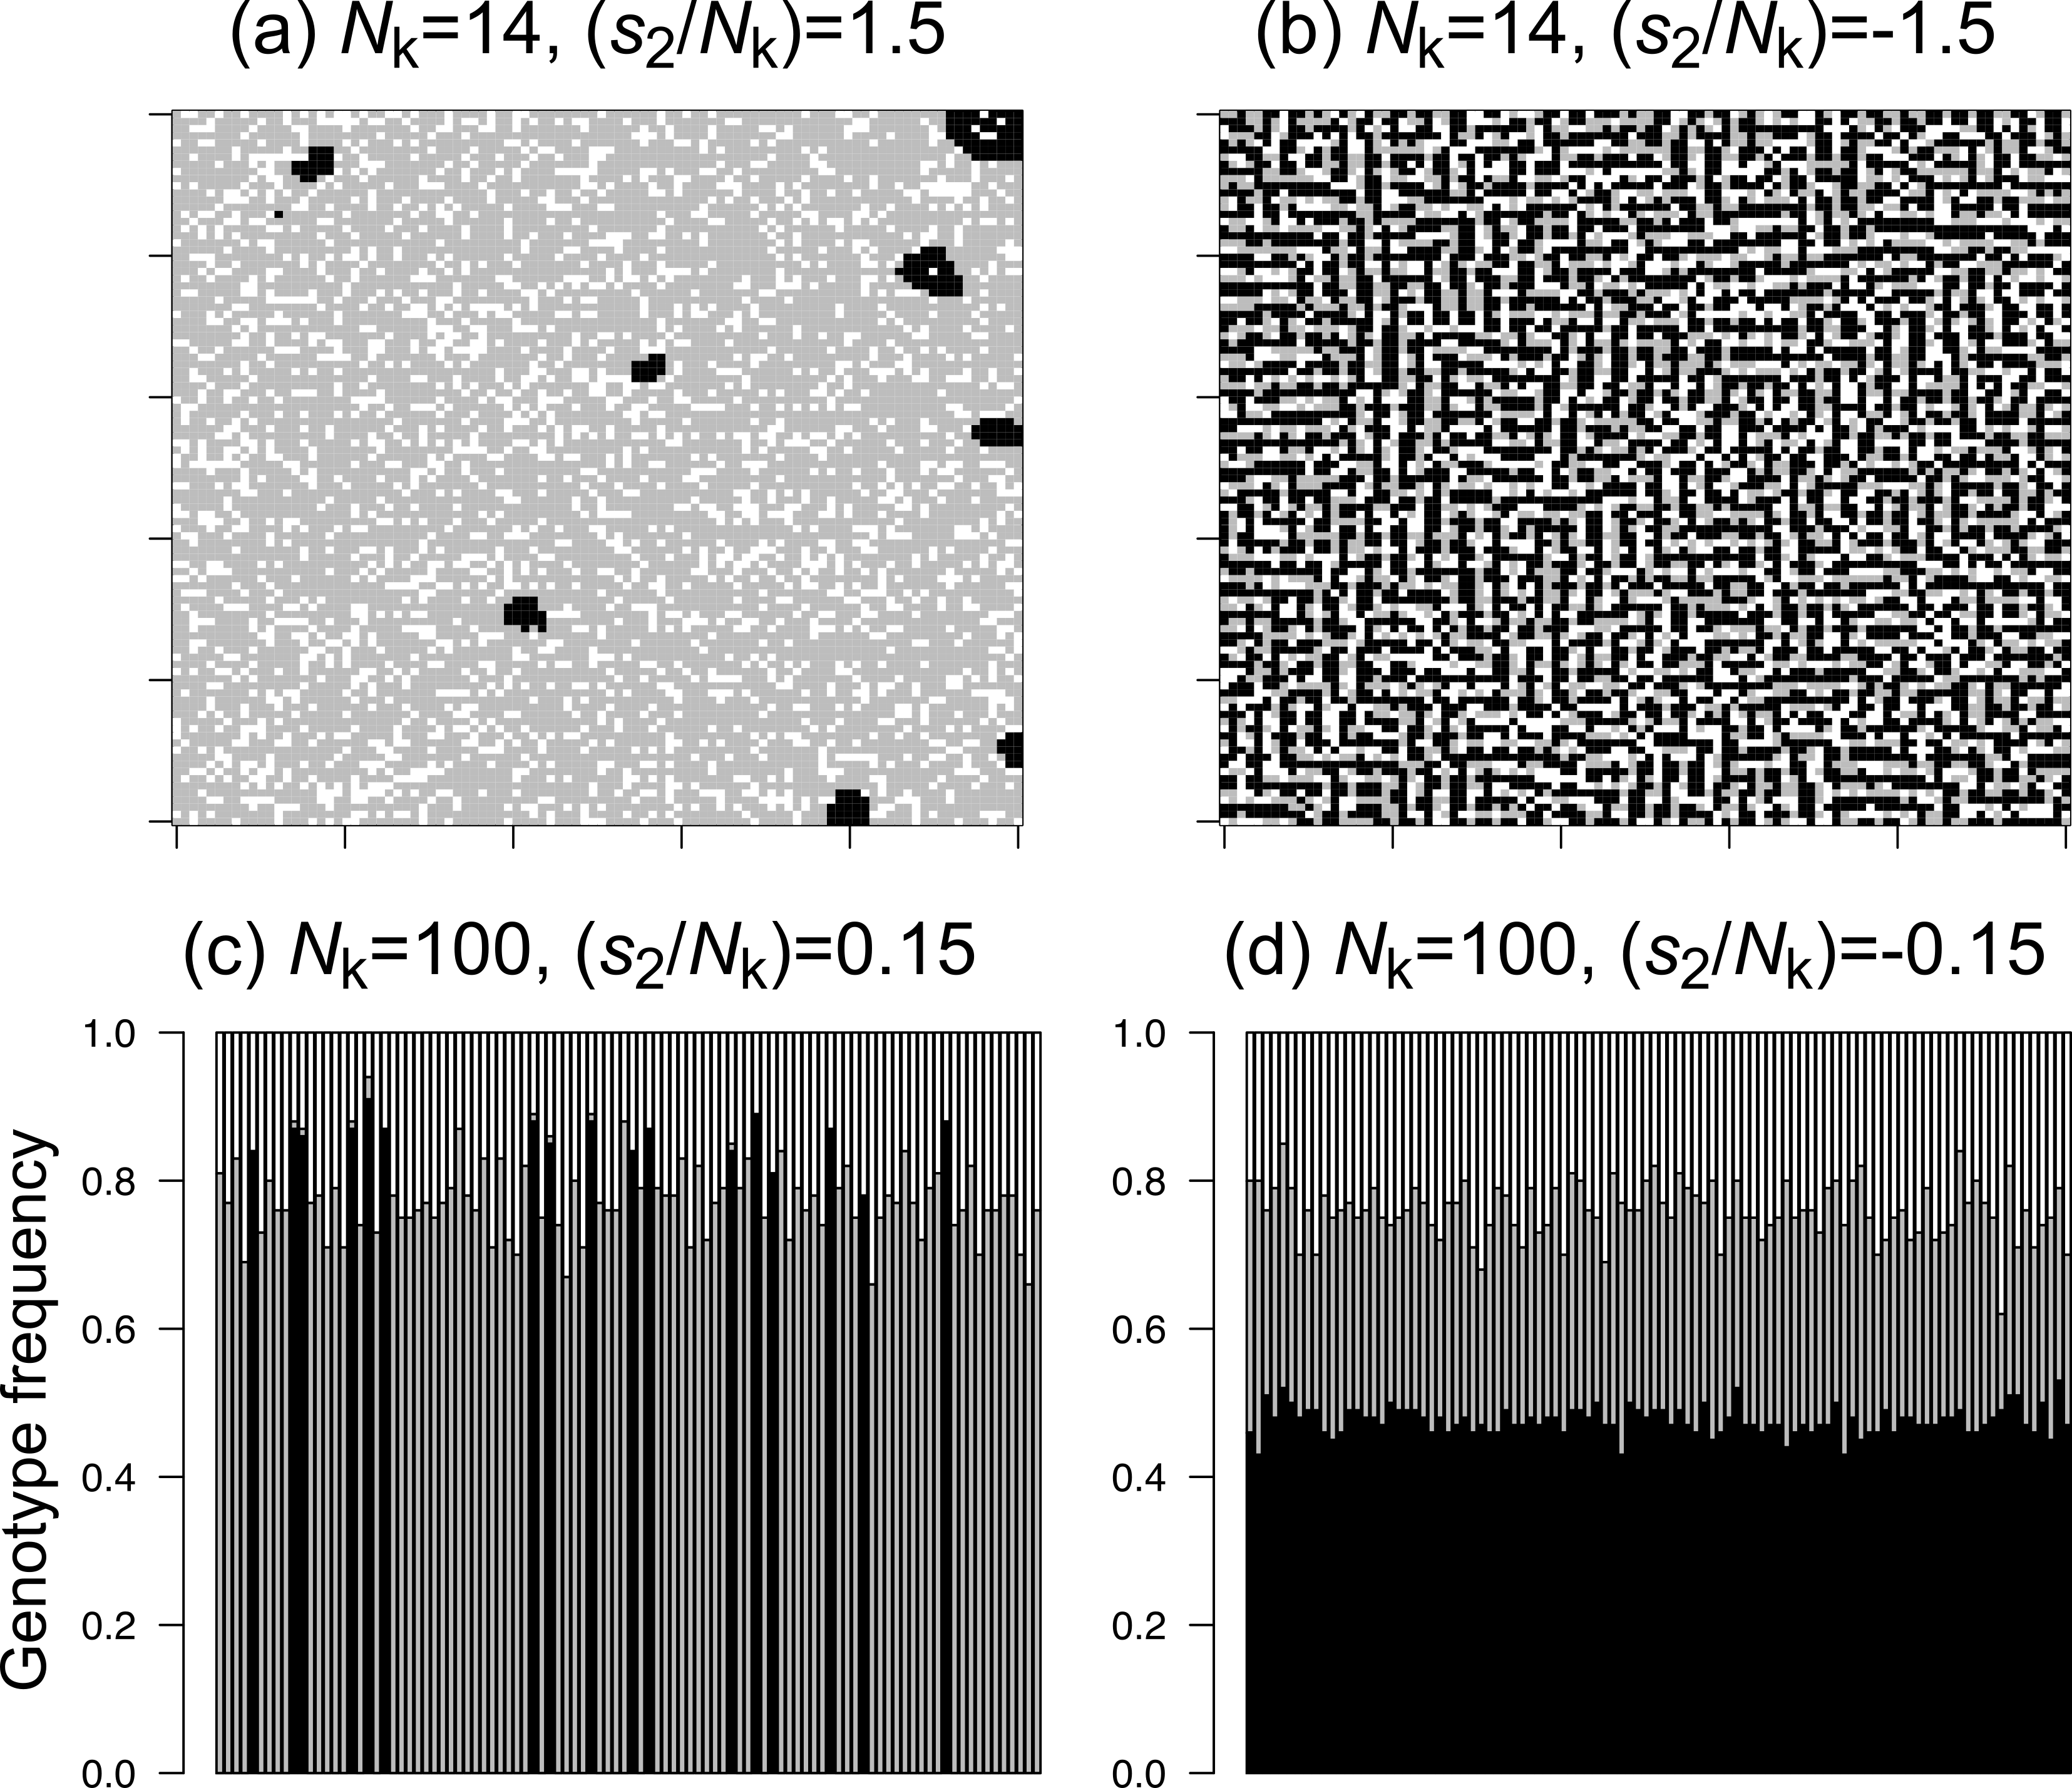
\includegraphics[width=0.8\linewidth]{IsingExample.png}
  \caption{Numerical simulations maximizing the fitness $w_1 = w_0 + s_1g_i + (s_2 / {N_k})\sum^{N_k}_{j=i}{g_ig_j}$ (Appendix S1) for 100 generations. White, gray, and black indicate the AA, Aa, and aa genotypes, respectively. Top panels (a, b) represent plant genotype distributions across a 100 $\times$ 100 continuous lattice space when interactions are restricted to the second nearest neighbors ($N_k=14$). Each grid corresponds to an individual. Bottom panels (c, d) represent the genotype frequencies among 100 split populations composed of 100 individuals each. Each vertical bar corresponds to a population. Left panels (a, c) simulate positive frequency-dependent selection (FDS), while right panels (b, d) simulate negative FDS. No directional selection were assumed as $w_0 = 0$ and $s_1 = 10^{-4}$ for all simulations, whereas the subpopulation size $N_k$ and interaction strength per individual $s_2/N_k$ were changed.}
  \label{figS1:Ising}
\end{figure}

\noindent
The probability of sampling AA, Aa, and aa at $t+1$ generation is denoted as $P_{\mathrm{AA},t+1}$, $P_{\mathrm{Aa},t+1}$, and $P_{\mathrm{aa},t+1}$, respectively. Let $f_\mathrm{AA}$, $f_\mathrm{Aa}$, and $f_\mathrm{aa}$ be the frequencies of genotypes AA, Aa, and aa within a population with $f_\mathrm{AA}$, $f_\mathrm{Aa}$, and $f_\mathrm{aa}$. In summary, the transition from generation $t$ to $t+1$ is expressed as

$$
\left( \begin{array}{cc} 
    P_{\mathrm{AA},t+1}\\ 
    P_{\mathrm{Aa},t+1}\\
    P_{\mathrm{aa},t+1}\\
    \end{array} \right) 
    =
\left(\begin{array}{ccc}
    (f_\mathrm{AA}+0.5f_\mathrm{Aa}) & (0.5f_\mathrm{AA}+0.25f_\mathrm{Aa}) & 0\\ 
    (f_\mathrm{aa}+0.5f_\mathrm{Aa}) & (0.5f_\mathrm{AA}+0.5f_\mathrm{Aa}+0.5f_\mathrm{aa}) & (f_\mathrm{AA}+0.5f_\mathrm{Aa})\\
    0 & (0.25f_\mathrm{Aa}+0.5f_\mathrm{aa}) & (0.5f_\mathrm{Aa}+f_\mathrm{aa})\\
    \end{array} \right) 
\left( \begin{array}{cc} 
    P_{\mathrm{AA},t}\\ 
    P_{\mathrm{Aa},t}\\
    P_{\mathrm{aa},t}\\
    \end{array} \right),
$$
\noindent
where the elements of the transition matrix were calculated from the three genotype frequencies and the segregation ratio of Mendelian inheritance. The zero elements pose a constraint where one homozygote cannot turn into another homozygote in a single generation. Given that the sum of the three genotype frequencies was 1 as $f_\mathrm{AA}+f_\mathrm{Aa}+f_\mathrm{aa}=1$, the probability of remaining as a heterozygote was 0.5. Therefore, the outcome from the modified Metropolis algorithm was expected to be qualitatively the same as a random proposal of three genotypes, but quantitatively different in the excess of heterozygotes within a population.

Figure \ref{figS1:Ising} shows the results of numerical simulations under continuous and split subpopulations with complete dominance as $g_i \in$ \{AA, Aa, aa\} $=$ \{+1, +1, -1\}. The three genotypes were well mixed and maintained in a continuous space when $s_2<0$ (Fig. \ref{figS1:Ising}b), whereas several clusters of the aa genotype were observed when $s_2>0$ (Fig. \ref{figS1:Ising}a). Three genotypes were also maintained at an intermediate frequency in a split space when $s_2<0$ (Fig. \ref{figS1:Ising}d), whereas the allele frequency was heavily biased when $s_2>0$ (Fig. \ref{figS1:Ising}c). The numerical simulations show that the sign of $s_2$ likely corresponded to the direction of the frequency-dependent selection (FDS) in a continuous and split space.

In summary, our Equation (\ref{eq:1}) based on genotype similarity represents negative and positive FDS with its selection coefficient $s_2$. By estimating $s_2$ from the individual fitness $w_i$, the regression model Equation (\ref{eq:2}) provided an empirical framework to detect FDS in the main text (see the methods "\textit{\textbf{Regression model of FDS}}").

\newpage
\clearpage
\medskip
\subsection*{Appendix S2. Fitness function under symmetric and asymmetric FDSs}
In this appendix, we show how our regression model can represent FDS under three cases of genotype encoding: complete dominance with random mating; additive effects with random mating; and asexual or inbred lines without mating. To analyze the regression model Equation (\ref{eq:3}) as a fitness function of allele frequency, we considered a single diallelic locus in an ideal population where diploid individuals were randomly mating and uniformly interacting in a sufficiently large population (i.e., $N \to \infty$). We also assumed no maternal or paternal effects on fitness such that the genotypes Aa and aA could not be distinguished. To concentrate on the mean trends of the model, we neglected the residuals as $e_i = 0$. Replacing $N_{k}$ into $N$, we redefined Equation (\ref{eq:3}) as follows:

\begin{equation}
y_i = \beta_0 + \beta_1x_i + \frac{\beta_2}{N}\sum^{N}_{j=1}{x_ix_j} + \frac{\beta_{12}x_i}{N}\sum^{N}_{j=1}{x_ix_j} \label{eq:s4}
\end{equation}
\noindent
where the trait value $y_i$ corresponds to the fitness value $w_i$ for individual $i$, the intercept $\beta_0$ corresponds to the base fitness $w_0$, the individual genotype coefficient $\beta_1$ corresponds to the directional selection coefficient $s_1$, and the coefficients $\beta_2$ and $\beta_{12}$ correspond to the selection coefficients related to FDS. The second term can also be transformed for simplicity as $\beta_2(\sum^{N}_{j=1}x_i x_j)/N = \beta_2x_i(\sum^{N}_{j=1}x_j)/N$, and the third term, $\beta_{12}x_i(\sum^{N}_{j=1}x_i x_j)/N = \beta_{12}x^2_i(\sum^{N}_{j=1}x_j)/N$. Provided $x^2_i=(-1)^2=1^2=1$, the third term represents a selection gradient due to the relative abundance of one allele in a neighborhood, irrespective of the individual genotype of a focal individual $i$.

We then transformed Equation (\ref{eq:s4}) into a function of the frequency of A alleles $f$, where the frequency of a alleles was defined conversely as $1-f$. When all the individuals were randomly interacting in a panmictic population, the interaction strength between $i$ and $j$ depended on the frequencies of AA, Aa, or aa genotypes derived from allele frequency. Thus, the fitness values of the three genotypes, $y_\mathrm{AA}(f)$, $y_\mathrm{Aa}(f)$, and $y_\mathrm{aa}(f)$, are functions of allele frequency $f$. For convenience, we suppressed the dependence on $f$, unless necessary. The ratio of AA, Aa, and aa genotypes within the panmictic population was given by AA:Aa:aa $=f^2: 2f(1-f)$: $(1-f)^2$. Assuming the aforementioned ideal population, we designated all combinations of interactions among AA, Aa, and aa genotypes and weighted the interactions based on their genotype frequencies. Table \ref{tableS2:intTable} lists the interaction strength weighted by the genotype frequency for symmetric and asymmetric effects. 

\begin{table}[h]
\caption{Cross tables showing the strength of interactions between the focal genotype $x_i$ and counterpart $x_j$ in a randomly interacting and mating population.}
(a) Symmetric effects \\
\begin{tabular}{|l|lll|}
\hline
$x_j$ \textbackslash{} $x_i$ & $x_\mathrm{AA}$ & $x_\mathrm{Aa}$ & $x_\mathrm{aa}$ \\ \hline
$x_\mathrm{AA}$ & $\beta_2 f^2x_\mathrm{AA}x_\mathrm{AA}$ & $\beta_2f^2x_\mathrm{Aa}x_\mathrm{AA}$ & $\beta_2f^2x_\mathrm{aa}x_\mathrm{AA}$ \\
$x_\mathrm{Aa}$ & $2\beta_2f(1-f)x_\mathrm{AA}x_\mathrm{Aa}$ & $2\beta_2f(1-f)x_\mathrm{Aa}x_\mathrm{Aa}$ & $2\beta_2f(1-f)x_\mathrm{aa}x_\mathrm{Aa}$ \\
$x_\mathrm{aa}$ & $\beta_2(1-f)^2x_\mathrm{AA}x_\mathrm{aa}$ & $\beta_2(1-f)^2x_\mathrm{Aa}x_\mathrm{aa}$ & $\beta_2(1-f)^2x_\mathrm{aa}x_\mathrm{aa}$ \\ \hline
\end{tabular}

\vspace*{5mm}

(b) Asymmetric effects \\
\begin{tabular}{|l|lll|}
\hline
$x_j$ \textbackslash{} $x_i$ & $x_\mathrm{AA}$ & $x_\mathrm{Aa}$ & $x_\mathrm{aa}$ \\ \hline
$x_\mathrm{AA}$ & $\beta_{12}f^2x^2_\mathrm{AA}x_\mathrm{AA}$  &  $\beta_{12}f^2x^2_\mathrm{Aa}x_\mathrm{AA}$  & $\beta_{12}f^2x^2_\mathrm{aa}x_\mathrm{AA}$ \\
$x_\mathrm{Aa}$ & $2\beta_{12}f(1-f)x^2_\mathrm{AA}x_\mathrm{Aa}$ & $2\beta_{12}f(1-f)x^2_\mathrm{Aa}x_\mathrm{Aa}$ &  $2\beta_{12}f(1-f)x^2_\mathrm{aa}x_\mathrm{Aa}$ \\
$x_\mathrm{aa}$ & $\beta_{12}(1-f)^2x^2_\mathrm{AA}x_\mathrm{aa}$ & $\beta_{12}(1-f)^2x^2_\mathrm{Aa}x_\mathrm{aa}$ & $\beta_{12}(1-f)^2x^2_\mathrm{aa}x_\mathrm{aa}$ \\ \hline
\end{tabular}
      \label{tableS2:intTable}
\end{table}

\noindent
Based on these cross tables (Table \ref{tableS2:intTable}), we redefined Equation (\ref{eq:s4}) for the three genotypes as: 

\begin{subequations} \label{eq:s5}
\begin{gather}
    \begin{split}
y_\mathrm{AA} &= \beta_0 + \beta_1x_\mathrm{AA} + \beta_2f^2x_\mathrm{AA}x_\mathrm{AA} + 2\beta_2f(1-f)x_\mathrm{AA}x_\mathrm{Aa} + \beta_2(1-f)^2x_\mathrm{AA}x_\mathrm{aa} \\
& + \beta_{12}f^2x^2_\mathrm{AA}x_\mathrm{AA} + 2\beta_{12}f(1-f)x^2_\mathrm{AA}x_\mathrm{Aa}+ \beta_{12}(1-f)^2x^2_\mathrm{AA}x_\mathrm{aa} \label{eq:s5a}
    \end{split}
\end{gather}
\begin{gather}
    \begin{split}
y_\mathrm{Aa} &= \beta_0 + \beta_1x_\mathrm{Aa} + \beta_2f^2x_\mathrm{Aa}x_\mathrm{AA} + 2\beta_2f(1-f)x_\mathrm{Aa}x_\mathrm{Aa} + \beta_2(1-f)^2x_\mathrm{Aa}x_\mathrm{aa} \\
& + \beta_{12}f^2x^2_\mathrm{Aa}x_\mathrm{AA} + 2\beta_2f(1-f)x^2_\mathrm{Aa}x_\mathrm{Aa}+ \beta_{12}(1-f)^2x^2_\mathrm{Aa}x_\mathrm{aa} \label{eq:s5b}
    \end{split}
\end{gather}
\begin{gather}
    \begin{split}
y_\mathrm{aa} &= \beta_0 + \beta_1x_\mathrm{aa} + \beta_2f^2x_\mathrm{aa}x_\mathrm{AA} + 2\beta_2f(1-f)x_\mathrm{aa}x_\mathrm{Aa} + \beta_2(1-f)^2x_\mathrm{aa}x_\mathrm{aa} \\
& + \beta_{12}f^2 x^2_\mathrm{aa}x_\mathrm{AA} + 2\beta_2f(1-f)x^2_\mathrm{aa}x_\mathrm{Aa}+ \beta_{12}(1-f)^2x^2_\mathrm{aa}x_\mathrm{aa} \label{eq:s5c}
    \end{split}
\end{gather}
\end{subequations}

\noindent
We further weighted the genotype-level fitness values by allele frequency. The allele-level fitness for A or a alleles is then given by:

\begin{subequations} \label{eq:s6}
\begin{align}
y_\mathrm{A} = fy_\mathrm{AA} + (1-f)y_\mathrm{Aa} \label{eq:s6a} \\
y_\mathrm{a} = fy_\mathrm{Aa} + (1-f)y_\mathrm{aa} \label{eq:s6b}
\end{align}
\end{subequations}

\noindent
The population-level mean fitness was finally defined by the weighted mean of the allele-level fitness as follows:

\begin{equation}
\begin{split}
\bar{y} &= fy_\mathrm{A} + (1-f)y_\mathrm{a} \\
&= f^2y_\mathrm{AA} + 2f(1-f)y_\mathrm{Aa} + (1-f)^2y_\mathrm{aa} \label{eq:s7}
\end{split}
\end{equation}

\noindent
Consequently, we could analyze fitness functions by inputting specific values in the three genotype values $x_\mathrm{AA}, x_\mathrm{Aa}$, and $x_\mathrm{aa}$ throughout Equations (\ref{eq:s5}) and (\ref{eq:s6}). In the following, we present three specific cases of complete dominance, additive effects, and asexual populations.

Case 1. Complete dominance with random mating: Novel mutations are expected to be recessive during adaptive evolution. Empirical studies have reported FDS on dimorphic traits that often exhibit complete dominance of one over another allele \citep[e.g.,][]{takahashi2010negative,sato2017herbivore,goldberg2020herbivore}. First, we considered the case in which the A alleles were completely dominant over a alleles, as encoded by $x_i \in$ \{AA, Aa, aa\} $=$ \{+1, +1, -1\}. Here, we neglected the directional selection as $\beta_1=0$ in Equation (\ref{eq:s5}) to focus on the fitness functions under FDS alone. Replacing the genotypes ($x_\mathrm{AA}$, $x_\mathrm{Aa}$, and $x_\mathrm{aa}$) according to their genotype values in Equation (\ref{eq:s5}) gave the fitness value to the three genotypes as

\begin{subequations}
\begin{gather}
    \begin{split}
y_\mathrm{AA} = y_\mathrm{Aa} &= \beta_0 + \beta_2 [(+1)\times(+1)] f^2 + \beta_2 [(+1)\times(+1)] 2f(1-f) + \beta_2 [(+1)\times(-1)] (1-f)^2 \\
& + \beta_{12} [(+1)^2\times(+1)] f^2 + \beta_{12} [(+1)^2\times(+1)] 2f(1-f) + \beta_{12} [(+1)^2\times(-1)] (1-f)^2 \\ 
&= \beta_0 + \beta_2(2f-1+2f-2f^2) + \beta_{12}(2f-1+2f-2f^2) \\
&= \beta_0 + (\beta_{12}+\beta_2)(4f-2f^2-1)~~~\mathrm{where}~x_\mathrm{AA}=x_\mathrm{Aa} = +1 \label{eq:s8a}
    \end{split}
\end{gather}
\begin{gather}
    \begin{split}
y_\mathrm{aa} &= \beta_0 + \beta_2[(-1)\times(+1)]f^2 + \beta_2[(-1)\times(+1)]2f(1-f) + \beta_2[(-1)\times(-1)](1-f)^2 \\
& + \beta_{12}[(-1)^2\times(+1)]f^2 + \beta_{12}[(-1)^2\times(+1)]2f(1-f) + \beta_{12}[(-1)^2\times(-1)](1-f)^2 \\ 
&= \beta_0 - \beta_2(2f-1+2f-2f^2) + \beta_{12}(2f-1+2f-2f^2) \\
&= \beta_0 + (\beta_{12}-\beta_2)(4f-2f^2-1)~~~\mathrm{where}~x_\mathrm{aa} = +1 \label{eq:s8b}
    \end{split}
\end{gather}
\end{subequations}

\noindent
The allele-level fitness following Equations (\ref{eq:s6a}) and (\ref{eq:s6b}) was given by 

\begin{subequations}
\begin{align}
y_\mathrm{A} = fy_\mathrm{AA} + (1-f)y_\mathrm{Aa} = fy_\mathrm{AA} + (1-f)y_\mathrm{AA} = y_\mathrm{AA} \label{eq:s9a} \\
y_\mathrm{a} = fy_\mathrm{Aa} + (1-f)y_\mathrm{aa} = y_\mathrm{aa} + 2f\beta_2(4f-2f^2-1) \label{eq:s9b}
\end{align}
\end{subequations}

\noindent
The relative fitness between A and a alleles was calculated as: $y_\mathrm{A} - y_\mathrm{a} = y_\mathrm{AA} - y_\mathrm{aa} - 2f\beta_2(4f-2f^2-1) = 2\beta_2(1-f)(4f-2f^2-1)$. Solving $y_\mathrm{A} - y_\mathrm{a} = 0$ with respect to $f$ within the range of (0,1) resulted in $f^*=-0.5\sqrt{2}+1$, which showed a single stable or unstable state within $f=(0,1)$ in the case of complete dominance under FDS. The population-level mean fitness is finally given by

\begin{equation}
\begin{split}
\bar{y} &= fy_\mathrm{A} + (1-f)y_\mathrm{a} \\
&= \beta_0 + (4f\beta_2-2f^2\beta_2-\beta_2+\beta_{12})(4f-2f^2-1) \label{eq:s10}
\end{split}
\end{equation}

\noindent
Figure \ref{fig2:asym} in the main text (see the methods "\textit{\textbf{Fitness function given by regression coefficients}}") shows the allele-level fitness [Equations (\ref{eq:s9a}) and (\ref{eq:s9b})] and population-level mean fitness [Equation (\ref{eq:s10})]. The mean fitness was maximized at a stable equilibrium at the intermediate allele frequency under symmetric negative FDS, whereas it was minimized at an unstable equilibrium under symmetric positive FDS. When asymmetric FDS and complete dominance are involved, equilibria do not always match the maxima or minima of the mean fitness because of the nonlinearity of the allele-level fitness in response to $f$. Still, the mean fitness at the stable or unstable point was higher or lower than expected compared with the weighted mean of the two monomorphic populations. A similar notion was suggested by a general model of FDS in population genetics \citep{cockerham1972frequency, schneider_maximization_2008}.

Case 2. Additive effects with random mating: Although few empirical studies have reported FDS on quantitative traits, this case is of theoretical interest in the general model of FDS \citep[e.g.,][]{schneider_maximization_2008}. Considering the fitness value as a quantitative trait, we then analyzed the additive effects of A and a alleles on $y_i$ as encoded by $x_i \in $ \{AA, Aa, aa\} $=$ \{+1, 0, -1\}. Replacing the genotypes ($x_\mathrm{AA}$, $x_\mathrm{Aa}$, and $x_\mathrm{aa}$) according to their genotype values in Equations (\ref{eq:s5}) gave the fitness value to the three genotypes as:

\begin{subequations}
\begin{gather}
    \begin{split}
y_\mathrm{AA} &= \beta_0 + \beta_2 [(+1)\times(+1)] f^2 + \beta_2 [(+1)\times(-1)] (1-f)^2 \\
& + \beta_{12} [(+1)^2\times(+1)] f^2 + \beta_{12} [(+1)^2\times(-1)] (1-f)^2 \\ 
&= \beta_0 + \beta_2f^2 - \beta_2(1-2f+f^2) + \beta_{12}f^2 - \beta_{12}(1-2f+f^2) \\
&= \beta_0 + \beta_2(2f - 1) + \beta_{12}(2f-1) \\ 
&= \beta_0 + (\beta_{12}+\beta_2)(2f-1)~~~\mathrm{where}~x_\mathrm{AA} = +1 \label{eq:s11a}
    \end{split}
\end{gather}
\begin{gather}
    y_\mathrm{Aa} = \beta_0~~~\mathrm{where}~x_\mathrm{Aa} = 0 \label{eq:s11b}
\end{gather}
\begin{gather}
    \begin{split}
y_\mathrm{aa} &= \beta_0 + \beta_2 [(-1)\times(+1)] f^2\ + \beta_2 [(-1)\times(+1)] (1-f)^2 \\
& + \beta_{12} [(-1)^2\times(+1)] f^2 + \beta_{12} [(-1)^2\times(-1)] (1-f)^2 \\
&= \beta_0 - \beta_2f^2 + \beta_2(1-2f+f^2) + \beta_{12}f^2 - \beta_{12}(1-2f+f^2) \\
&= \beta_0 - \beta_2(2f - 1) + \beta_{12}(2f-1) \\
&= \beta_0 + (\beta_{12} - \beta_2)(2f - 1)~~~\mathrm{where}~x_\mathrm{aa} = -1 \label{eq:s11c}
    \end{split}
\end{gather}
\end{subequations}

\noindent
The fitness function for the two homozygotes AA and aa [i.e., Equations (\ref{eq:s5a}) and (\ref{eq:s5c})] turned out to be linear in response to $f$. The allele-level fitness following Equations (\ref{eq:s6a}) and (\ref{eq:s6b}) is then given by:

\begin{subequations}
\begin{gather}
    \begin{split}
y_\mathrm{A} &= fy_\mathrm{AA} + (1-f)y_\mathrm{Aa}\\
&= \beta_0+f(\beta_{12}+\beta_2)(2f-1) \label{eq:s12a}
    \end{split}
\end{gather}
\begin{gather}
    \begin{split}
y_\mathrm{a} &= fy_\mathrm{Aa} + (1-f)y_\mathrm{aa}\\
&= \beta_0+(1-f)(\beta_{12}-\beta_2)(2f-1) \label{eq:s12b}
    \end{split}
\end{gather}
\end{subequations}

\noindent
The relative fitness was calculated as $y_\mathrm{A} - y_\mathrm{a} = (2f-1)[f(\beta_{12}+\beta_2) - (1-f)(\beta_{12}-\beta_2)] = (2f-1)(2\beta_{12}f-\beta_{12}+\beta_2)$. Solving $y_\mathrm{A} - y_\mathrm{a} = 0$ with respect to $f$ within a range of (0,1) yields $f^*=0.5$ and $f^*=0.5(\beta_{12}-\beta_2)/\beta_{12}$, showing that the additive action of FDS made multiple equilibria possible at the intermediate allele frequency within $f = (0,1)$. The mean fitness following Equation (\ref{eq:s7}) is finally given by:

\begin{equation}
\begin{split}
\bar{y} &= fy_\mathrm{A} + (1-f)y_\mathrm{a} \\
&= \beta_0 + f^2(\beta_{12}+\beta_2)(2f-1) + (1-f)^2(\beta_{12}-\beta_2)(2f-1)\\
&= \beta_0 + (2f-1)[2f^2(\beta_{12}+\beta_2)-2f(\beta_{12}-\beta_2)+\beta_{12}-\beta_2] \label{eq:s13}
\end{split}
\end{equation}

\begin{figure}[ht]
  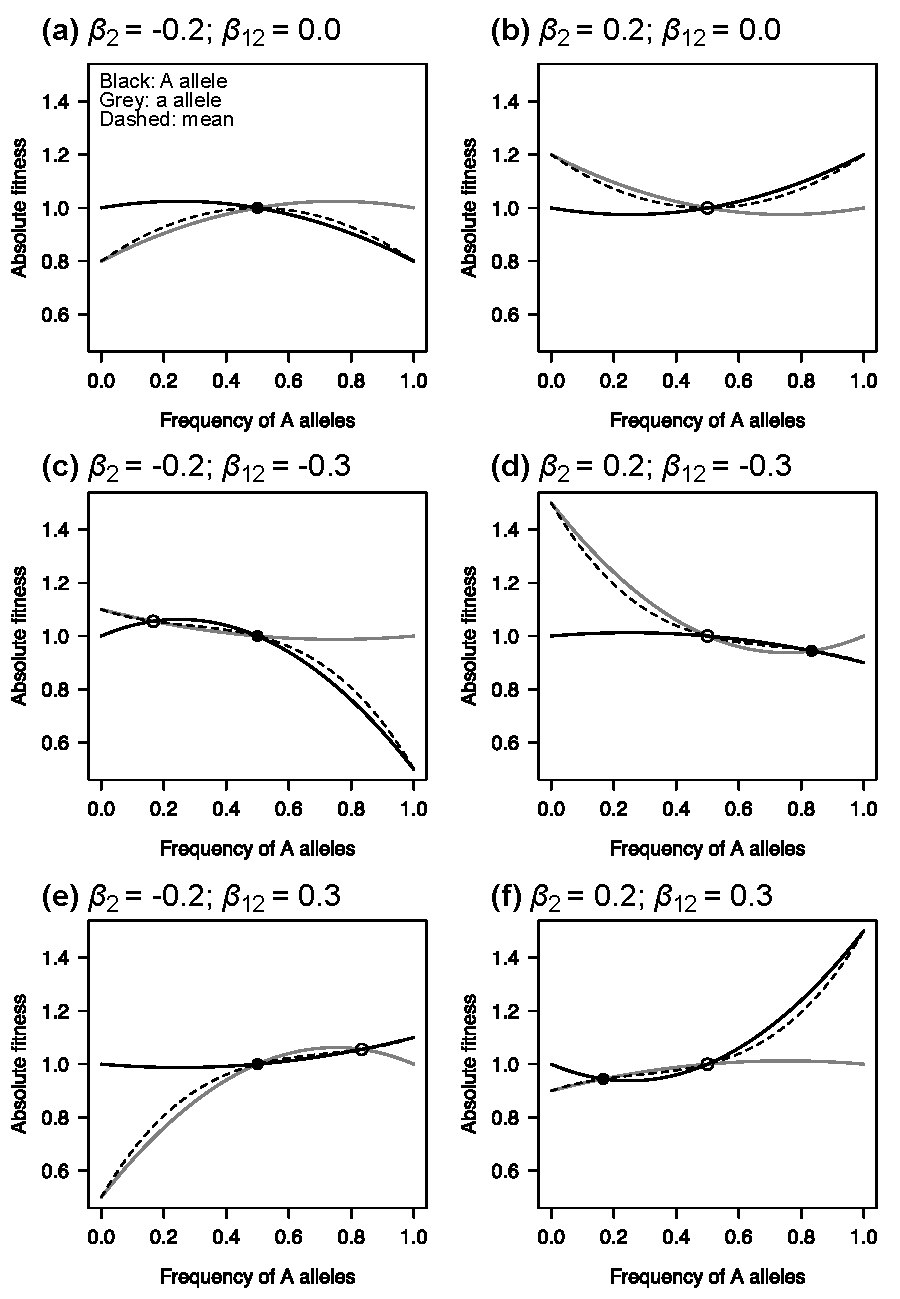
\includegraphics[width=0.95\linewidth]{AsymFDSadd.pdf}
  \caption{Numerical examples for the fitness values $y_i$ in response to allele frequency when A and a alleles have additive effects on the fitness; that is, Equations (\ref{eq:s12a}) and (\ref{eq:s12b}) in Appendix S2. Black and gray lines indicate the allele-level fitness of the A or a allele, respectively. The dashed curves indicate the mean fitness per population; that is, Equation (\ref{eq:s13}) in Appendix S2. (a) Symmetric negative frequency-dependent selection (FDS); (d) symmetric positive FDS; (b and c) asymmetric negative FDS; and (e and f) asymmetric positive FDS. Closed and open circles indicate a stable or unstable state, respectively. No directional selection i.e., $\beta_0=1.0$ and $\beta_1=0$ are assumed for all panels to present fitness functions of FDS.}
  \label{figS2:FDSadd}
\end{figure}

Figure \ref{figS2:FDSadd} shows numerical examples of the allele-level fitness [Equations (\ref{eq:s12a}) and (\ref{eq:s12b})] and the mean fitness [Equation (\ref{eq:s13})] in response to $f$. Similar to the case of complete dominance, the mean fitness was maximized or minimized at a stable or unstable equilibrium under the symmetric FDS (Fig. \ref{figS2:FDSadd}a and d). In contrast, a stable and unstable equilibrium occurred simultaneously under asymmetric FDS (Fig. \ref{figS2:FDSadd}b-c and e-f), where the maxima or minima of mean fitness did not always match the equilibria. This potential of multiple equilibria was also suggested by a one-locus two-allele model of FDS when it involved asymmetric FDS \citep{schneider_maximization_2008}. 

Case 3. Asexual or inbred lines without mating: In common gardens or laboratory experiments, researchers arbitrarily distribute inbred accessions in space and retrieve individuals before mating \citep[e.g.,][]{sato2019neighbor}. This was also the case for the field GWAS experiment in the main text. Furthermore, ecological studies often focus on FDS at the phenotype level with asexual reproduction assumed \citep[e.g.,][]{takahashi2018balanced}. In these cases, heterozygotes were negligible, and the two homozygotes were encoded as $x_i \in $ \{AA, aa\} $=$ \{+1, -1\} \citep{sato2019neighbor}. Let $f_\mathrm{AA}$ and $f_\mathrm{aa}$ be the frequency of AA and aa genotypes within a population, where $f_\mathrm{AA} + f_\mathrm{aa} = 1$. The fitness function for the AA or aa genotype is given by:

\begin{subequations}
\begin{gather}
    \begin{split}
y_\mathrm{AA} &= \beta_0 + \beta_2f_\mathrm{AA}[(+1)\times(+1)] + \beta_2(1-f_\mathrm{AA})[(+1)\times(-1)] \\
&+ \beta_{12}f_\mathrm{AA}[(+1)^2\times(+1)] + \beta_{12}(1-f_\mathrm{AA})[(+1)^2\times(-1)] \\ 
&= \beta_0 + \beta_2(2f_\mathrm{AA}-1) + \beta_{12}(2f_\mathrm{AA}-1) \\ 
&= \beta_0 + (\beta_{12}+\beta_2)(2f_\mathrm{AA}-1)~~~\mathrm{where}~x_\mathrm{AA} = +1 \label{eq:s14a}
    \end{split}
\end{gather}
\begin{gather}
    \begin{split}
y_\mathrm{aa} &= \beta_0 + \beta_2f_\mathrm{AA}[(-1)\times(+1)] + \beta_2(1-f_\mathrm{AA})[\times(-1)\times(-1)] \\
&+ \beta_{12}f_\mathrm{AA}[(-1)^2\times(+1) + \beta_{12}(1-f_\mathrm{AA})[(-1)^2\times(-1)] \\
&= \beta_0 - \beta_2(2f_\mathrm{AA}-1) + \beta_{12}(2f_\mathrm{AA}-1) \\
&= \beta_0 + (\beta_{12}-\beta_2)(2f_\mathrm{AA}-1)~~~\mathrm{where}~x_\mathrm{aa} = -1 \label{eq:s14b}
    \end{split}
\end{gather}
\end{subequations}

\noindent
where the population-level mean fitness was given by its weighted mean as follows. 

\begin{equation}
\begin{split}
\bar{y} &= f_\mathrm{AA}y_\mathrm{AA} + (1-f_\mathrm{AA})y_\mathrm{aa} \\
&= f_\mathrm{AA}(y_\mathrm{AA}-y_\mathrm{aa}) + y_\mathrm{aa} \\
&= 2\beta_{2}f_\mathrm{AA}(2f_\mathrm{AA}-1) + (\beta_{12}-\beta_2)(2f_\mathrm{AA}-1) + \beta_0 \label{eq:s15}
\end{split}
\end{equation}

Figure \ref{figS3:FDSinbred} shows the fitness function of the AA or aa genotype [Equations (\ref{eq:s14a}) and (\ref{eq:s14b})] and population mean [Equation \ref{eq:s15}]. The fitness function of the two homozygotes was the same as that of the additive case described above. The mean fitness became simpler as the allele frequency corresponded to the genotype frequency. As this inbred case represented two genotypes with asexual reproduction, its conclusion was basically the same as that derived from game theoretical models \citep{takahashi2018balanced}. 

In Figure \ref{fig3:GLMM}, we present this inbred case with $\beta_1 \neq 0$, where the genotype fitness Equations (\ref{eq:s14a}) and (\ref{eq:s14b}) is rewritten as

\begin{subequations}
\begin{align}
    y_\mathrm{AA} = \beta_0 + \beta_1 + (\beta_{12}+\beta_2)(2f_\mathrm{AA}-1) \label{eq:s16a} \\
    y_\mathrm{aa} = \beta_0 - \beta_1 + (\beta_{12}-\beta_2)(2f_\mathrm{AA}-1) \label{eq:s16b}
\end{align}
\end{subequations}

\noindent
where the relative fitness is given by $y_\mathrm{AA} - y_\mathrm{aa} = 2\beta_1 + 2\beta_2(2f_\mathrm{AA}-1)$. Solving $y_\mathrm{AA} - y_\mathrm{aa} = 0$ with respect to $f_\mathrm{AA} = (0,1)$ yields $f^*_\mathrm{AA} = 1 - 0.5\beta_1 / \beta_2$. Therefore, the directional selection coefficient $\beta_1$ may modify the equilibrium. When $\beta_1 \neq 0$, the mean fitness Equation (\ref{eq:s15}) can also be rewritten as:

\begin{equation}
\begin{split}
\bar{y} &= f_\mathrm{AA}y_\mathrm{AA} + (1-f_\mathrm{AA})y_\mathrm{aa} \\
&= 2\beta_{2}f_\mathrm{AA}(2f_\mathrm{AA}-1) + (\beta_{12}-\beta_2)(2f_\mathrm{AA}-1) + 2f\beta_1 - \beta_1 + \beta_0 \label{eq:s16}
\end{split}
\end{equation}

\begin{figure}[ht]
  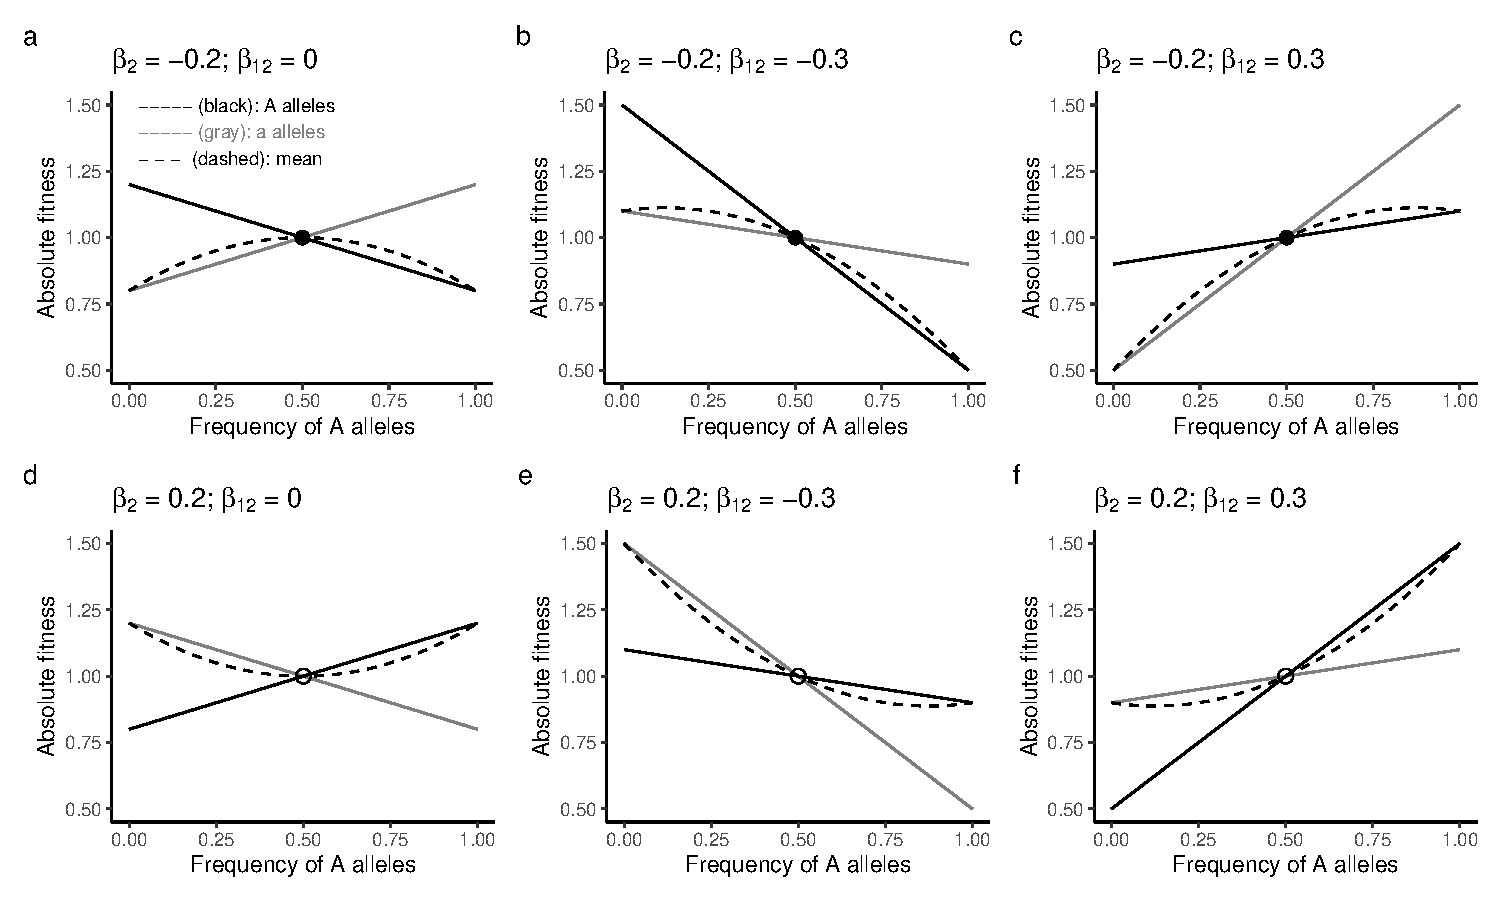
\includegraphics[width=0.95\linewidth]{AsymFDSinbred.pdf}
  \caption{Numerical examples of fitness values $y_i$ in response to allele frequency when only the AA and aa genotypes exist without mating [Equations (\ref{eq:s14a}) and (\ref{eq:s14b}) in Appendix S2]. Black and gray lines indicate the fitness functions for the AA and aa genotypes, respectively. The dashed curves indicate the mean fitness per population; that is, Equation (\ref{eq:s15}) in Appendix S2. (a) Symmetric negative frequency-dependent selection (FDS); (d) symmetric positive FDS; (b and c) asymmetric negative FDS; and (e and f) asymmetric positive FDS. Closed and open circles indicate a stable or unstable state, respectively. No directional selection i.e., $\beta_0=1.0$ and $\beta_1=0$ are assumed for all panels to present fitness functions of FDS.}
  \label{figS3:FDSinbred}
\end{figure}

\newpage
\clearpage
\medskip
\subsection*{Appendix S3. Mixed model extension}
To implement GWAS, we modified Equations (\ref{eq:2}) and (\ref{eq:3}) as a linear mixed model (LMM) that considered genetic relatedness as a random effect \citep{kang2008efficient}. In terms of Henderson's mixed model \citep{henderson1959estimation}, such GWAS models have the same structure as phylogenetic comparative methods that analyze interspecific phenotypic variation among phylogenetic trees \citep{kang2008efficient, hadfield2010general}. To modify Equation (\ref{eq:2}) as a LMM, we designated the genetic-related matrix as $\mathbf{A}$ and introduced random effects $u_i$ to Equation (\ref{eq:2}) as follows: 

\begin{equation}
y_i = \beta_0 + \beta_1x_i + \beta_2\sum^{N_{k}}_{j=1}{x_ix_j} + u_i + e_i \label{eq:s1}
\end{equation}
\noindent
where a vector including $u_i$ for $n$ individuals followed a normal distribution as $u_i \in \mathbf{u}$ and $\mathbf{u} \sim$ Norm($\mathbf{0}$, $\sigma^2_1\mathbf{A}_1+\sigma^2_2\mathbf{A}_2$). The residual $e_i$ is expressed as $e_i \in \mathbf{e}$ and $\mathbf{e} \sim$ Norm($\mathbf{0}$, $\sigma^2_e\mathbf{I}$).
The $n$ × $n$ variance–covariance matrices denote the individual genetic relatedness or the entire genotype similarity among $n$ individuals as
$\mathbf{A}_1=\frac{1}{2(q-1)}\mathbf{X}_1^\mathsf{T}\mathbf{X}_1 + \frac{1}{2}$ and 
$\mathbf{A}_2=\frac{1}{(q-1)}\mathbf{X}_2^\mathsf{T} \mathbf{X}_2$,
where $q$ denotes the number of loci. The elements of $n$ individuals $\times$ $q$ loci matrix $\mathbf{X}_1$ consist of explanatory variables of the individual genotype values. As we defined $x_i = (-1, 1)$, the genetic-related matrix $\mathbf{A}_1$ was scaled to represent the proportion of loci shared among $n$ × $n$ individuals. The elements of $n$ individuals $\times$ $q$ loci matrix $\mathbf{X}_2$ consist of the genotype similarity as:

$$\mathbf{X}_2=\left(\begin{array}{cccc}
    (\sum^{N_k}_{j=1}x_{1,1} x_j)/N_k &  (\sum^{N_k}_{j=1}x_{1,2} x_j)/N_k &  ... &  (\sum^{N_k}_{j=1}x_{1,n} x_j)/N_k \\ 
    (\sum^{N_k}_{j=1}x_{1,2} x_j)/N_k &  (\sum^{N_k}_{j=1}x_{2,2} x_j)/N_k &  ... &  (\sum^{N_k}_{j=1}x_{2,n} x_j)/N_k\\
    ... & ... & ... & ... \\
    (\sum^{N_k}_{j=1}x_{q,1} x_j)/N_k &  (\sum^{N_k}_{j=1}x_{q,2} x_j)/N_k &  ... &  (\sum^{N_k}_{j=1}x_{q,n} x_j)/N_k \\
    \end{array} \right)
$$

\noindent
where the $n \times n$ matrix $\mathbf{A}_2$ indicates a sample structure related to genotype similarity. The variance component parameters $\sigma^2_1$ and $\sigma^2_2$ determine the relative contributions of $\mathbf{A}_1$ and $\mathbf{A}_2$ to the vector of random effects $\mathbf{u}$.

To incorporate asymmetric FDS into GWAS, we considered a sample structure based on the asymmetric FDS in LMM. Here, we extended Equation (\ref{eq:3}) into LMM as

\begin{equation}
y_i = \beta_0 + \beta_1x_i + \frac{\beta_2}{N_k}\sum^{N_{k}}_{j=1}{x_ix_j} + \frac{\beta_{12}x_i}{N_k}\sum^{N_{k}}_{j=1}{x_ix_j} + u_i + e_i \label{eq:s2}
\end{equation}
\noindent
where the random effect $u_i$ is redefined as $u_i \in \mathbf{u}$ and $\mathbf{u} \sim$ Norm($\mathbf{0}$, $\sigma^2_1\mathbf{A}_1+\sigma^2_2\mathbf{A}_2+\sigma^2_{12}\mathbf{A}_{12}$). The additional $n \times n$ variance-covariance matrix $\mathbf{A}_{12}$ denotes a sample structure because of the asymmetric effects among $n$ individuals as $\mathbf{A}_{12}=\frac{1}{(q-1)}\mathbf{X}_{12}^\mathsf{T} \mathbf{X}_{12}$. The elements of $n$ individuals $\times$ $q$ loci matrix $\mathbf{X}_{12}$ consist of explanatory variables for the asymmetric effects as follows:

$$\mathbf{X}_{12}=\left(\begin{array}{cccc}
    (x_{1,1}\sum^{N_k}_{j=1}x_{1,1} x_j)/N_k &  (x_{1,2}\sum^{N_k}_{j=1}x_{1,2} x_j)/N_k &  ... &  (x_{1,n}\sum^{N_k}_{j=1}x_{1,n} x_j)/N_k \\ 
    (x_{1,2}\sum^{N_k}_{j=1}x_{1,2} x_j)/N_k &  (x_{2,2}\sum^{N_k}_{j=1}x_{2,2} x_j)/N_k &  ... &  (x_{2,n}\sum^{N_k}_{j=1}x_{2,n} x_j)/N_k\\
    ... & ... & ... & ... \\
    (x_{q,1}\sum^{N_k}_{j=1}x_{q,1} x_j)/N_k &  (x_{q,2}\sum^{N_k}_{j=1}x_{q,2} x_j)/N_k &  ... &  (x_{q,n}\sum^{N_k}_{j=1}x_{q,n} x_j)/N_k \\
    \end{array} \right)
$$
The additional parameter of the variance component $\sigma^2_{12}$ compares the relative importance of the asymmetric effects with those of the individual genotype effects $\sigma^2_1$ and genotype similarity effects $\sigma^2_2$.
Additionally, the individual-level formula Equation (\ref{eq:s2}) can also be converted into a common matrix form \citep{henderson1959estimation} as follows:

\begin{equation}
    \mathbf{y}=\mathbf{X}\bm{\beta}+\mathbf{Zu}+\mathbf{e} \label{eq:s3}
\end{equation}

\noindent
where $\mathbf{y}$ is $n \times 1$ fitness vector with $y_i \in \mathbf{y}$; $\mathbf{X}$ is a matrix of fixed effects, including a unit vector, individual genotype $x_i$, genotype similarity covariate $(\sum^{N_k}_{j=1}x_i x_j)/N_k$, and other covariates for $n$ individuals; $\bm{\beta}$ is a vector that included coefficients of the fixed effects; $\mathbf{Z}$ is a design matrix allocating individuals to a genotype; $\mathbf{u}$ is the random effect as Var($\mathbf{u}$) $=\sigma^2_1\mathbf{A}_1+\sigma^2_2\mathbf{A}_2+\sigma^2_{12}\mathbf{A}_{12}$; and $\mathbf{e}$ is the residual as Var($\mathbf{e}$) $=\sigma^2_e\mathbf{I}$. 

To efficiently solve LMMs, we first estimated $\sigma^2_1$ and $\sigma^2_2$ without any fixed effects (i.e., null model) using the average-information restricted maximum likelihood (AI-REML) method implemented in the gaston package \citep{R_gaston}. Then, to compare the significance of $\beta_1$ and $\beta_2$ to the null model, we solved Equation (\ref{eq:s3}) using fast approximation by eigenvalue decomposition on a random effect matrix $\hat{\sigma}^2_1\mathbf{A}_1+\hat{\sigma}^2_2\mathbf{A}_2+\hat{\sigma}^2_{12}\mathbf{A}_{12}$. The likelihood ratio test was used to compare the models with and without $\beta_2$. The standard GWAS is a subset of Equation (\ref{eq:s1}) when $\beta_2=0$ and $\sigma^2_2=0$ \citep{sato2019neighbor}; thus, we set $\beta_2$ and $\sigma^2_2$ to zero when testing $\beta_1$. From results of this standard GWAS, we can also estimate the genomic heritability as $h^2=\hat{\sigma}^2_1/(\hat{\sigma}^2_1 + \hat{\sigma}^2_e)$. Because the individual genotype variable $x_i$ and the genotype similarity variable $(\sum^{N_{k}}_{j=1}{x_ix_j})/N_k$ were strongly correlated when the MAF was very small \citep{sato2019neighbor}, likelihood ratio tests should be performed one-by-one for each parameter in Equations (\ref{eq:s1}) and (\ref{eq:s2}). Such stepwise likelihood ratio tests were implemented using the rNeighborGWAS package version 1.2.4 \citep{sato2019neighbor}. The nei\_lmm() function was used for both the GWAS simulation and data analysis. The "asym = TRUE" option was used when testing the asymmetric effects $\beta_{12}$.


\newpage
\clearpage
\medskip
\subsection*{Appendix S4. Details of the GWAS simulation}
We performed simulations as summarized in the main text to examine the statistical power of the linear mixed model Equation (\ref{eq:s1}) in GWAS (see the methods "\textit{\textbf{GWAS of simulated data}}"). The entire procedure consisted of three steps: We simulated genomic structure under four different scenarios of selection (see "\textbf{Simulated genomes}" below), conducted virtual experiments to simulate fitness from the simulated genomes (see "\textbf{Virtual experiments}" below), and applied our method for the GWAS of simulated fitness and genomes (see "\textbf{GWAS using simulated genomes and fitness}" below). 

\subsubsection*{Simulated genomes}
To generate a realistic genome structure, we performed population genetic simulations using SLiM version 3 \citep{haller_slim_2019}. By running 30 independent iterations for 2000 generations, we simulated 50 kb nucleotide $\times$ three chromosomes $\times$ 10 subpopulations $\times$ 200 individuals. Base parameters were set as follows: mutation rate $\mu = 10^{-6}$, selection coefficient $s_1=s_2=0.1$ for non-neutral mutations, and recombination rate $r=10^{-5}$. Ten subpopulations were distributed in a circle with a low migration rate $m=10^{-4}$ between neighboring populations. In this simulation, we decomposed the total fitness as $w_i = w_{i,1} + w_{i,2}$. The first fitness component $w_{i,1}$ involves individual genotype effects $\beta_1$, and $w_{i,2}$ is the second fitness component subject to the power analysis of genotype similarity effects $\beta_2$. For individual genotype effects $\beta_1$, we define stabilizing selection as $w_{i,1} = 1.5 - [(z_{i,1} - z_1^*)^2 / s_1N_k]$, where $z_1^*$ is the optimum number of QTLs responsible for individual genotype effects per genome per population and $z_i$ is the number of QTLs for individual $i$. We set $z_1^*$ to 5 and assumed additive effects by the QTLs. Following the standard way to simulate polygenic selection \citep{haller_slim_2019}, we did not substitute QTLs for $w_{1,i}$ even after they were fixed. For the genotype similarity effects $\beta_2$, we assumed four specific scenarios of selection on the second fitness component $w_{i,2}$ as follows: 

Scenario 1. Negative frequency-dependent selection: For the test of $\beta_2$, we first simulated negative FDS on the second fitness component $w_{i,2}$. We simulated negative FDS for the second fitness component as $w_{i,2} = 1.5 - s_ 2 g _if_k$, where $f_k$ indicates the frequency of the mutation within a subpopulation $k$. Novel mutations were assumed to be recessive to ancestral alleles with genotype $g_i$ redefined as $g_i \in$ \{AA, Aa, aa\} $=$ \{1, 1, 0\}. Polymorphisms were likely balanced under negative FDS; thus, the mutation rate was set at half of the base parameter to maintain the number of causal SNPs in the same order as that in the other scenario.

Scenario 2. Positive frequency-dependent selection: We also simulated the opposite regime to negative FDS i.e., positive FDS on the second fitness component $w_{i,2}$. It is known that locally acting positive FDS within a subpopulation can lead to global coexistence of two alleles among subpopulations \citep{molofsky2001coexistence}. Therefore, we separated the entire population into four panmictic subpopulations to simulate polymorphic loci. Similar to the simulation of negative FDS, we simulated positive FDS as $w_{i,2} = 1.5 + s_ 2 g _if_k$. Novel mutations were assumed to be recessive to ancestral alleles with genotype $g_i$ redefined as $g_i \in$ \{AA, Aa, aa\} $=$ \{1, 1, 0\}. 

Scenario 3. Overdominance: To test whether $\beta_2$ confounded frequency-independent types of balancing selection, we simulated genomes under overdominance selection. The second fitness component is defined as $w_{i,2} = 1.5 + s_2hg_i$, where $h$ is the dominance coefficient expressed on the basis of genotypes as \{$h_\mathrm{AA}, h_\mathrm{Aa}, h_\mathrm{aa}$\} $=$ \{1.0, 2.0, 1.0\}.

Scenario 4. Spatiotemporally varying selection: To test another type of frequency-independent balancing selection, we simulated genomes under spatiotemporally varying selection. The second fitness component is defined as $w_{i,2} = 1.5 + s g_i$, where $s$ varies in space and time. We assumed $s_2=0.1$ for two subpopulations, and $s_2=-0.1$ for the other two subpopulations. For six of the four subpopulations, we changed the selection coefficient in time to $s_2=0.1$ for odd generations and $s_2=-0.1$ for even generations. We reset $m=0.001$ to allow a higher migration rate that could ensure spatially varying selection. In this scenario, novel mutations were assumed to be recessive to ancestral alleles.

\begin{figure}[ht]
  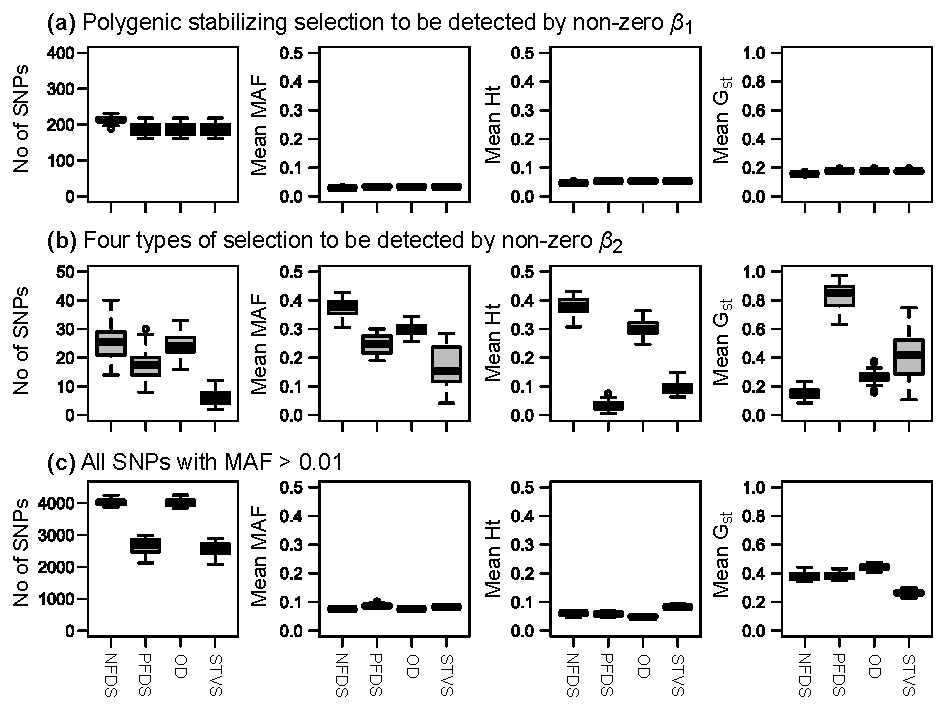
\includegraphics[width=\linewidth]{SimGenomeSummary.pdf}
  \caption{Structure of simulated genomes regarding the loci responsible for stabilizing selection (a), the other forms of selection (b), and genome-wide single nucleotide polymorphisms [SNPs](c). Number of SNPs, mean minor allele frequency (MAF), mean heterozygosity (\textit{H}\textsubscript{t}), and mean fixation indices (\textit{G}\textsubscript{st}) are shown among 30 iterations for four scenarios of selection: NFDS, negative frequency-dependent selection; PFDS, positive frequency-dependent selection; OD, overdominance; STVS, spatiotemporally varying selection.}
  \label{figS4:GenStr}
\end{figure}

As a result, the simulated genomes had 2,000 to 4,500 SNPs with MAFs $>$ 0.01 across 50 kbp nucleotide sequences (Fig. \ref{figS4:GenStr}). They exhibited low heterozygosity (\textit{H}\textsubscript{t} $<$ 0.1) and moderate to strong differentiation among 10 populations (\textit{G}\textsubscript{st} $<$ 0.5; Fig. \ref{figS4:GenStr}c), where approximately 200 SNPs were involved in polygenic stabilizing selection (Fig. \ref{figS4:GenStr}a). Regarding the causal SNPs, SNPs responsible for positive FDS showed strong population genetic structures (\textit{G}\textsubscript{st} $>$ 0.8) with low heterozygosity (\textit{H}\textsubscript{t} $<$ 0.05; Fig. \ref{figS4:GenStr}b) because positive FDS reduces polymorphisms within a population. In contrast, since negative FDS maintains polymorphisms within a population, SNPs responsible for negative FDS had weak population genetic structures (\textit{G}\textsubscript{st} $<$ 0.2) with high heterozygosity (\textit{H}\textsubscript{t} $>$ 0.35; Fig. \ref{figS4:GenStr}b).


\subsubsection*{Virtual experiments}
To simulate individual fitness, we sampled the simulated genomes and generated fitness values from the genotype data. The simulated genomes were exported in variant call format (.vcf) and loaded into R with the gaston \citep{R_gaston} and the vcfR package \citep{knaus2017vcfr}. SNPs were filtered with a cut-off threshold of a minor allele frequency (MAF) of 0.01. We tested two experimental settings: split and continuous populations (Fig. \ref{fig1:scheme}a). To describe the two distinct cases, 900 individuals were randomly sampled from each simulation without replacement and assigned to a 30 $\times$ 30 lattice space for the continuous setting, or 10 individuals each to 90 split cages for the split setting.

Fitness values were then simulated from the simulated genomes and their spatial arrangement. To calculate the individual genotype component $\beta_1x_i$ in Equation (\ref{eq:2}), we assigned 0.1 (which corresponded to the selection coefficient $s_1$ in the population genetic simulation) to $\beta_1$ of causal SNPs or zero to those of the other SNPs. The second fitness component at causal SNPs was generated with $\beta_2 = 0.1$ (corresponding to the strength of balancing selection $s_2$ in the population genetic simulation) for negative or positive FDS as $(\pm \beta_2\sum^{N_{k}}_{j=1}{x_ix_j}) / 2N_k$, for overdominance as $x_i \in$ \{AA, Aa, aa\} = \{$1+\beta_2, 1+\beta_2h, 1$\}, and for spatiotemporally varying selection as a random assignment of $\pm \beta_2$ to $\beta_2x_i$. Fitness variance was not adjusted for the first and second fitness components since the number of causal SNPs and their effect sizes were controlled during the population genetic simulation above. Gaussian residual errors were finally added to the simulated fitness such that approximately one-third of the total phenotypic variation was attributed to the environmental variance as Var($\mathbf{e}$) $=(0.75)^2 \times$Var($\mathbf{w}$). This range of the number of causal SNPs and the proportion of phenotypic variation explained by the model were based on parameter settings where the model performance was well differentiated \citep{sato2019neighbor}.

\begin{figure}[ht]
  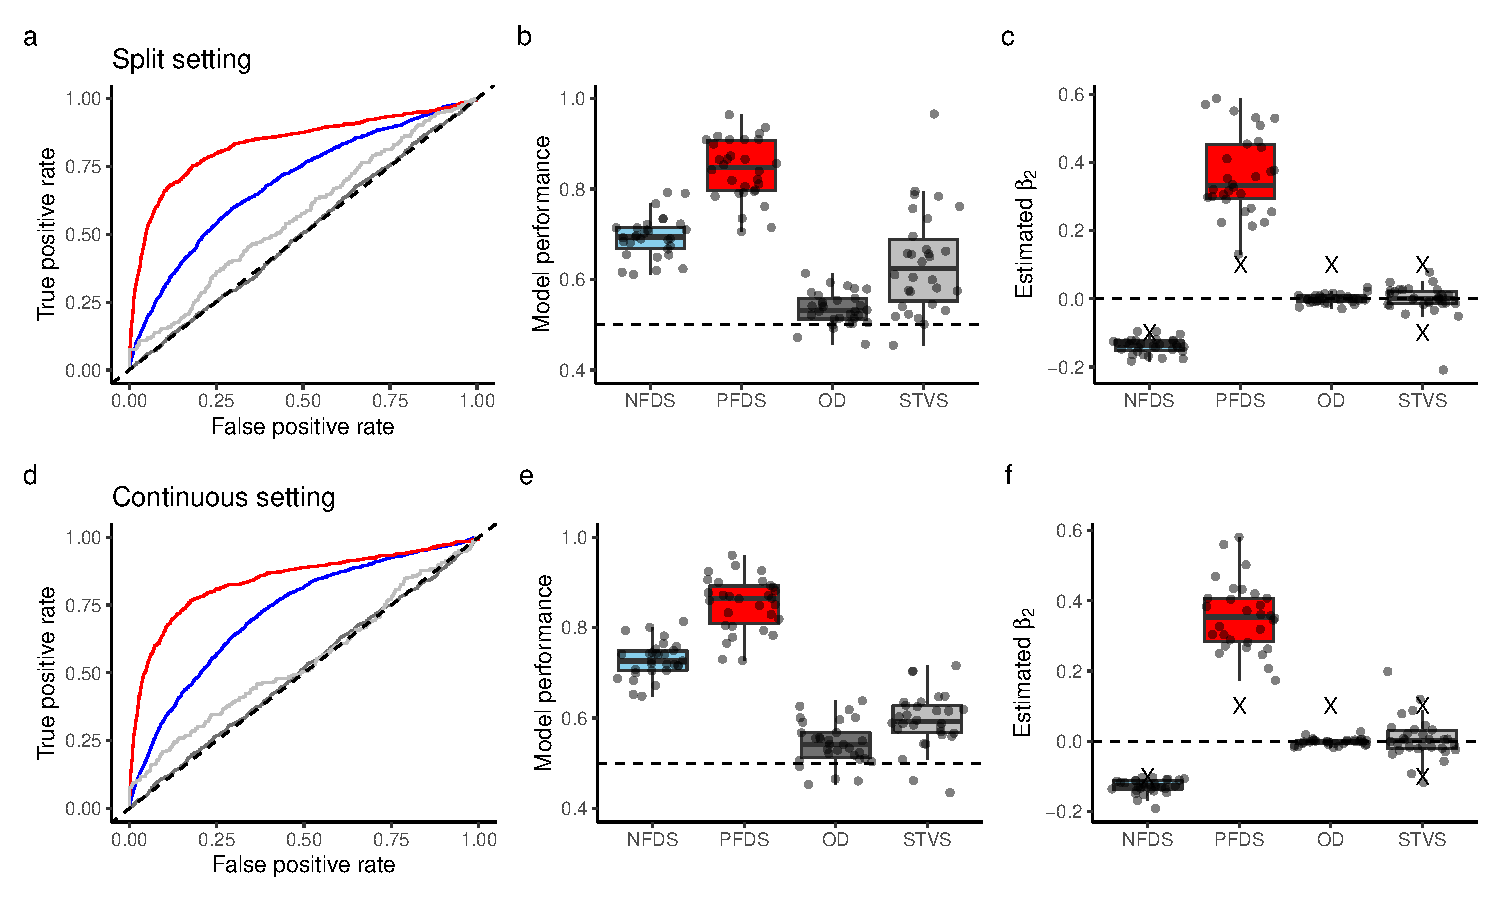
\includegraphics[width=0.85\linewidth]{beta2LMdomi.pdf}
  \caption{Performance of standard linear models to estimate the four types of simulated selections: NFDS, negative frequency-dependent selection; PFDS, positive frequency-dependent selection; OD, overdominance; and STVS, spatiotemporally varying selection. The complete dominance of A alleles over a alleles was assumed in this simulation. The top and bottom panels show the results of the split and continuous settings, respectively (Fig. \ref{fig1:scheme}a). (a and d) The receiver operating characteristic (ROC) curve shows the relationship between the true and false positive rate. Line colors indicate different simulation scenarios (blue, NFDS; red, PFDS; black, OD; gray, STVS). (b and e) Model performance evaluated by the area under the ROC curve (AUC). Dashed lines at 0.5 indicate no power to detect causal single nucleotide polymorphisms (SNPs). (c and f) Estimated $\beta_2$ of causal SNPs, where negative and positive values indicate negative and positive FDS, respectively. Cross marks indicate the true simulated magnitude of $\beta_2$.}
  \label{figS5:beta2LM}
\end{figure}

\begin{figure}[ht]
  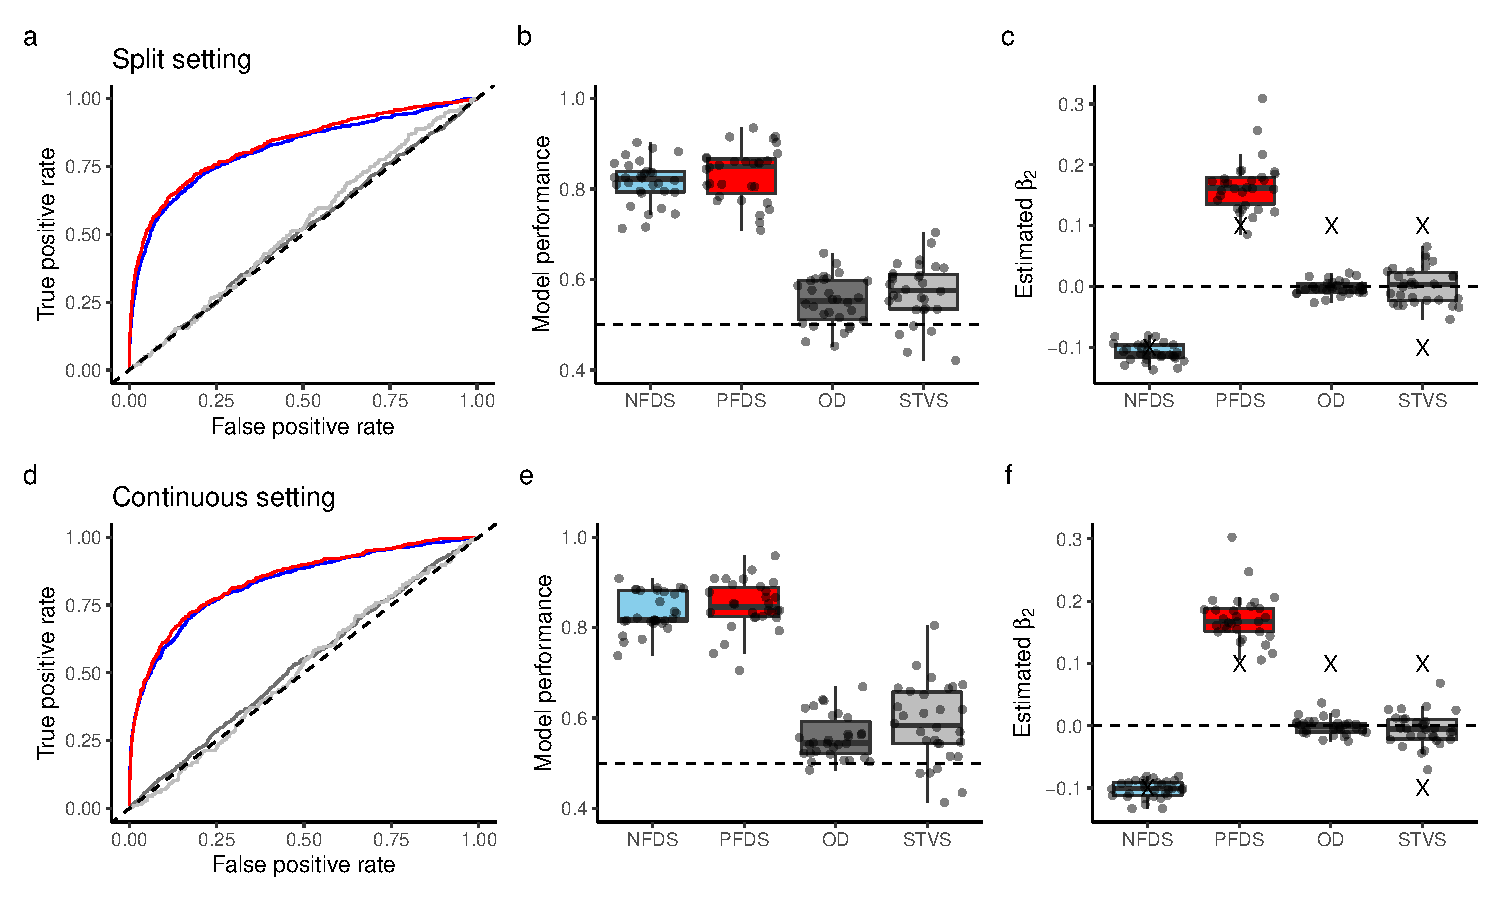
\includegraphics[width=0.85\linewidth]{beta2LMMadd.pdf}
  \caption{Performance of linear mixed models to estimate the four types of simulated selections: NFDS, negative frequency-dependent selection; PFDS, positive frequency-dependent selection; OD, overdominance; and STVS, spatiotemporally varying selection. The additive effects of two alleles on fitness were assumed in this simulation. The top and bottom panels show the results of the split and continuous settings, respectively (Fig. \ref{fig1:scheme}a). (a and d) Receiver operating characteristic (ROC) curves showing the relationship between the true and false positive rates. Line colors indicate different simulation scenarios (blue, NFDS; red, PFDS; black, OD; gray, STVS). (b and e) Model performance evaluated by the area under the ROC curve (AUC). Dashed lines at AUC = 0.5 indicate no power to detect causal single nucleotide polymorphisms (SNPs). (c and f) Estimated $\beta_2$ of causal SNPs, where negative and positive values indicate negative and positive FDS, respectively. Cross marks indicate the true simulated magnitude of $\beta_2$.}
  \label{figS:beta2LMMadd}
\end{figure}

\subsubsection*{GWAS using simulated genomes and fitness}
We performed association mapping with respect to $\beta_1$ and $\beta_2$ to detect FDS from the simulated fitness and genomes. The rNeighborGWAS package \citep{sato2019neighbor} was used to implement the regression model in Equation (\ref{eq:2}) as an LMM (Appendix S2). The false vs. true positive rates were analyzed using the receiver operating characteristic (ROC) curve. Like the generative model, we assumed the dominant encoding for the three genotypes, $x_i \in$ \{AA, Aa, aa\} $=$ \{+1, +1, -1\}. We calculated the area under the ROC curve (AUC) for the -log\textsubscript{10}($p$-values) of $\beta_1$ or $\beta_2$ to quantify the efficiency of causal polymorphism detection. The AUC ranged from 0.5 (no power to detect causal SNPs) to 1.0 (perfect matching between the top $p$-value score and causal SNPs). We compared the true and estimated values of $\beta_2$ to quantify the accuracy of the effect size estimates. We also compared AUCs and $\hat{\beta}_2$ between LMM and LM to test whether LMMs could outperform standard LMs.

\begin{figure}[ht]
  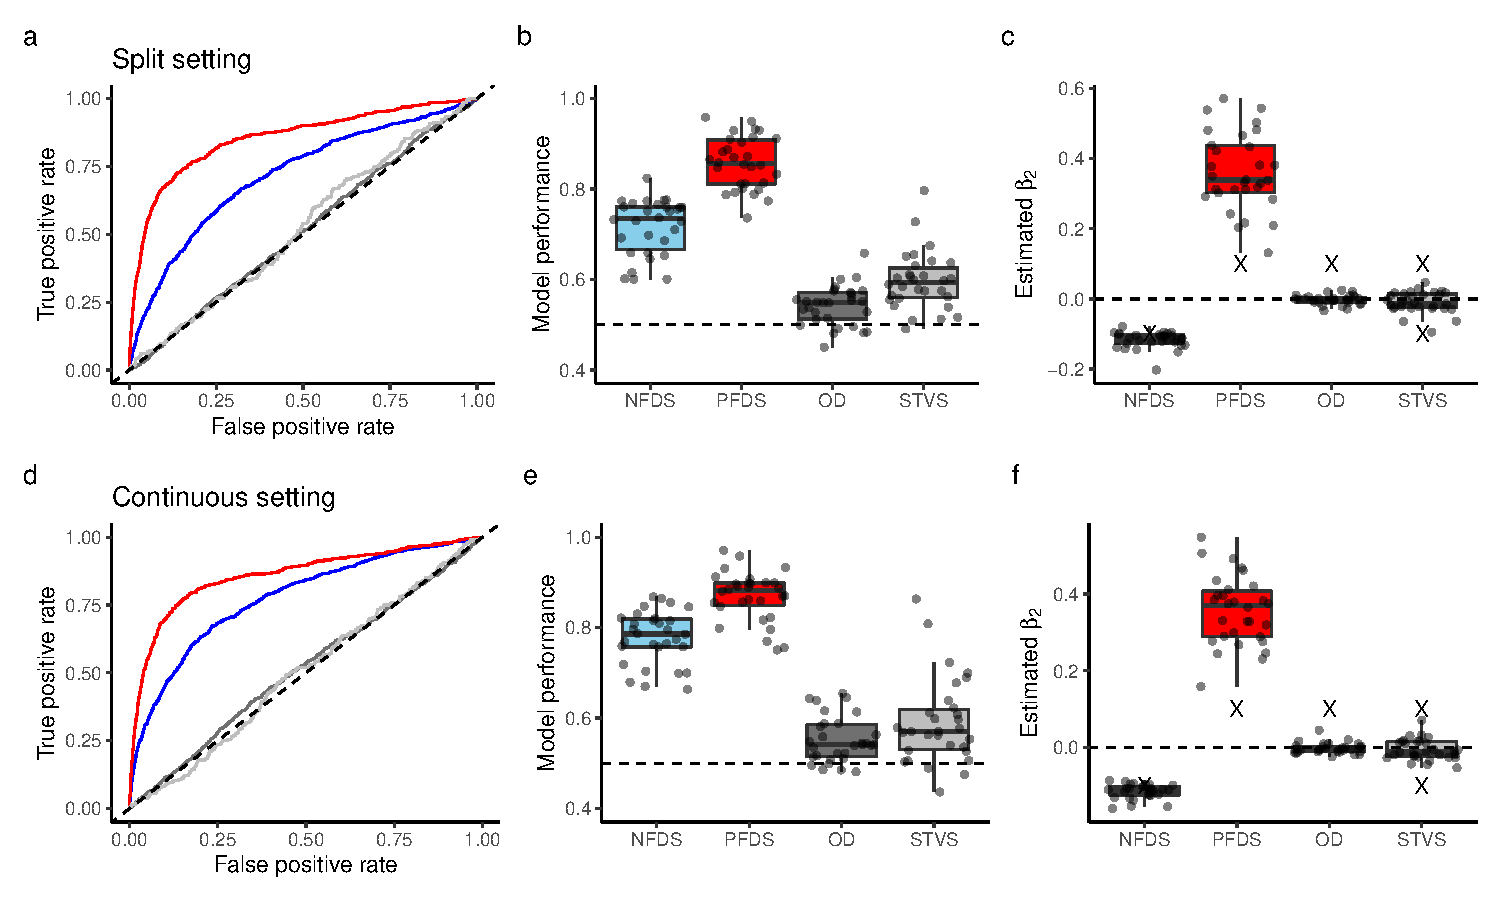
\includegraphics[width=0.85\linewidth]{beta2LMadd.pdf}
  \caption{Performance of standard linear models to estimate the four types of simulated selections: NFDS, negative frequency-dependent selection; PFDS, positive frequency-dependent selection; OD, overdominance; and STVS, spatiotemporally varying selection. The additive effects of two alleles on fitness were assumed in this simulation. The top and bottom panels show the results of the split and continuous settings, respectively (Fig. \ref{fig1:scheme}a). (a and d) Receiver operating characteristic (ROC) curve, which indicates the relationship between the true and false positive rate. Line colors indicate different simulation scenarios (blue, NFDS; red, PFDS; black, OD; gray, STVS). (b and e) Model performance evaluated by the area under the ROC curve (AUC). Dashed lines at AUC = 0.5 indicate no power to detect causal single nucleotide polymorphisms (SNPs). (c and f) Estimated $\beta_2$ of causal SNPs, where negative and positive values indicate negative and positive FDS, respectively. Cross marks indicate the true simulated magnitude of $\beta_2$.}
  \label{figS:beta2LMadd}
\end{figure}

Figure \ref{fig4:beta2LMM} presented the results when we assumed the complete dominance of A alleles over a allele. Figure \ref{fig4:beta2LMM} showed the effectiveness of linear mixed models (LMMs) for estimating the positive and negative FDS. Further, we find that LMMs outperform standard linear models (LMs) in terms of the efficient detection of causal SNPs (cf. Fig. \ref{fig4:beta2LMM}b, e and Fig. \ref{figS5:beta2LM}b, e) and the correct estimation of $\beta_2$ (cf. Fig. \ref{fig4:beta2LMM}c, f and Fig. \ref{figS5:beta2LM}c, f). Yet, researchers often assume the additive effects of two alleles on quantitative traits such as fitness, in GWAS \citep[e.g,][]{gondro2013genome,R_gaston}. Therefore, we examined the case of additive genotype encoding in this appendix. With the same simulation setting above, we fitted Equation (\ref{eq:2}) to the simulated fitness with the additive genotype encoding as $g_i \in$ \{AA, Aa, aa\} $=$ \{+1, 0, -1\}. Under this assumption of the additive effects, Figure \ref{figS:beta2LMMadd} or \ref{figS:beta2LMadd} present the results of LMMs or LMs, respectively. The LMMs retain high performance to detect both negative and positive FDS (median performance > 0.8: Fig. \ref{figS:beta2LMMadd}) and show better performance than LMs to detect negative FDS (Fig. \ref{figS:beta2LMMadd}b, e; \ref{figS:beta2LMadd}b, e). Although LMs and LMMs show similar performances in detecting positive FDS (Fig. \ref{figS:beta2LMMadd}b, e; \ref{figS:beta2LMadd}b, e), the positive coefficient of $\hat{\beta}_2$ is more overestimated in LMs than in LMMs (Fig. \ref{figS:beta2LMMadd}c, f; \ref{figS:beta2LMadd}c, f). These additional simulations suggest that LMMs are still preferred over LMs to suppress the overestimation and false positives.

\newpage
\clearpage
\medskip
\subsection*{Appendix S5. Details of GWAS experiment using \textit{A. thaliana}}
We measured the number of reproductive branches of \textit{Arabidopsis thaliana} accessions to perform GWAS using empirical data, as summarized in the main text (see the methods "\textit{\textbf{GWAS using field-grown Arabidopsis thaliana}}"). According to \cite{sato2019plant}, we established a summer cohort composed of natural accessions with various life cycles to investigate the survival and reproduction under stressful environments. We used 199 worldwide accessions (Table \ref{tableS3:GWASdata}) out of 2029 inbred lines genotyped by the RegMap \citep{horton_genome-wide_2012} and 1001 Genomes project \citep{alonso-blanco_1135_2016}. For the 199 accessions, 1,819,577 SNPs were selected at a cut-off threshold of MAF $>$ 0.05. The seeds of the 199 accessions were sown on Jiffy-seven (33 mm in diameter) and stratified under constant dark conditions at a temperature of 4C$^{\circ}$ for 1 week. Germinated seedlings were then grown under a short-day condition (8 hours light: 16 h dark, 20C$^{\circ}$) for 6 weeks to keep all the accession in the vegetative stage. Individual plants with Jiffy-pots were then potted into a new plastic pot (6 cm in diameter) filled with mixed soils of agricultural compost (Profi Substrat Classic CL ED73, Einheitserde Co.) and perlite with a 3:1 L ratio of perlite. Potted plants were transferred to the common garden at the Irchel Campus of the University of Zurich (Zurich, Switzerland: 47$^\circ$23$^\prime$N, 08$^\circ$33$^\prime$E) on 8 July 2019. In the field setting, a set of 199 accessions and an additional Col-0 accession were randomly assigned to each block without replacement. The 200 plants were set in plastic trays (10 $\times$ 40 cells in a continuous space) in a checkered pattern, which made each individual have four neighbors (i.e., $N_k = 4$). Three replicates of each randomized block were set $>$ 1.5 m apart from each other. Of 561 plants, 181 bolted 2 weeks after they were transferred to the field. The genomic heritability of the reproductive branch number was as high as $h^2 = 0.68$, which indicates a genetic control of this trait.

We depicted quantile-quantile plots (QQ plots) between the expected and observed association score of -log\textsubscript{10}($p$-value) to inspect whether the population genetic structure was corrected well. An ideal pattern is that only the top-scoring SNPs have far higher association score than expected. For example, \ref{figS9:QQplotLMM}c exhibited an almost flat association score as randomly expected, but only several highest-scoring SNPs had higher observed score than expected. If the observed association scores are higher than that randomly expected all across the SNPs, there is likely a confounding variable such as a population genetic structure that is responsible for such an inflation of $p$-values (e.g., Fig. \ref{figS11:QQplotLM}a). In this context, QQ plots of LMMs are as flat as observed association scores exhibit almost randomly expected association scores for $\beta_2$ and $\beta_{12}$ at -log\textsubscript{10}($p$-value) < 5 (Fig. \ref{figS9:QQplotLMM}b, c). In contrast, LMs show larger scores of -log\textsubscript{10}($p$-value) than LMMs (Fig. \ref{figS10:gwasLM}a-c; Fig. \ref{fig5:gwas}a-c) and their QQ plot exhibits a large or slight inflation of the association score (Fig. \ref{figS11:QQplotLM}). The association score of the individual genotype effects $\beta_1$ are severely inflated than randomly expected (Fig. \ref{figS11:QQplotLM}a). These diagnostic analyses support the notion that LMMs are better than LMs to analyze empirical GWAS data.

\begin{figure}[]
  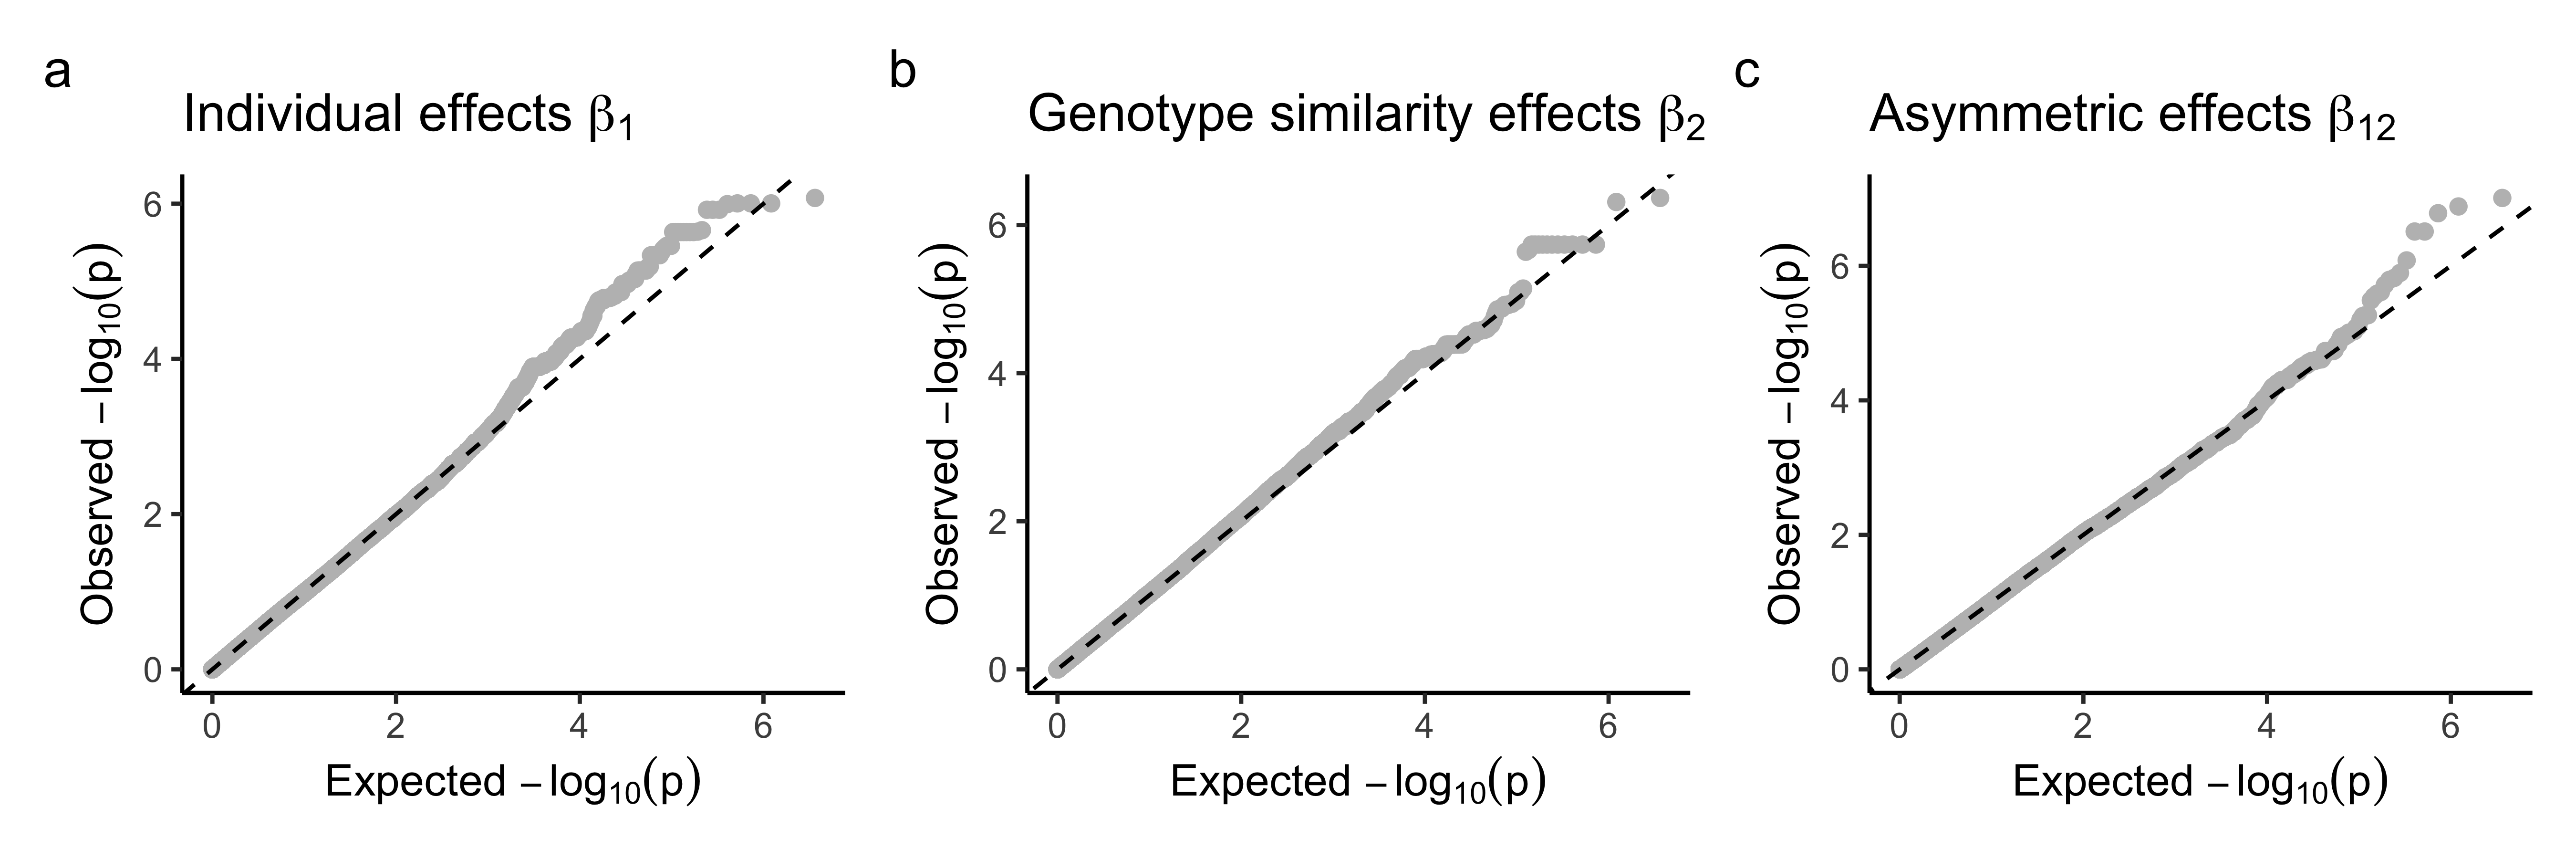
\includegraphics[width=\linewidth]{QQplotLMM.png}
  \caption{Quantile-quantile plots showing the observed and expected association score of the -log\textsubscript{10}($p$-values) for the genome-wide association studies of the reproductive branch number in field-grown \textit{A. thaliana}. The results obtained using the linear mixed models are shown. The left (a), middle (b), and right (c) panels display individual genotype, genotype similarity, and asymmetric effects, respectively. Dashed lines indicate the identity between the observed and expected association scores.}
  \label{figS9:QQplotLMM}
\end{figure}

\begin{figure}[]
  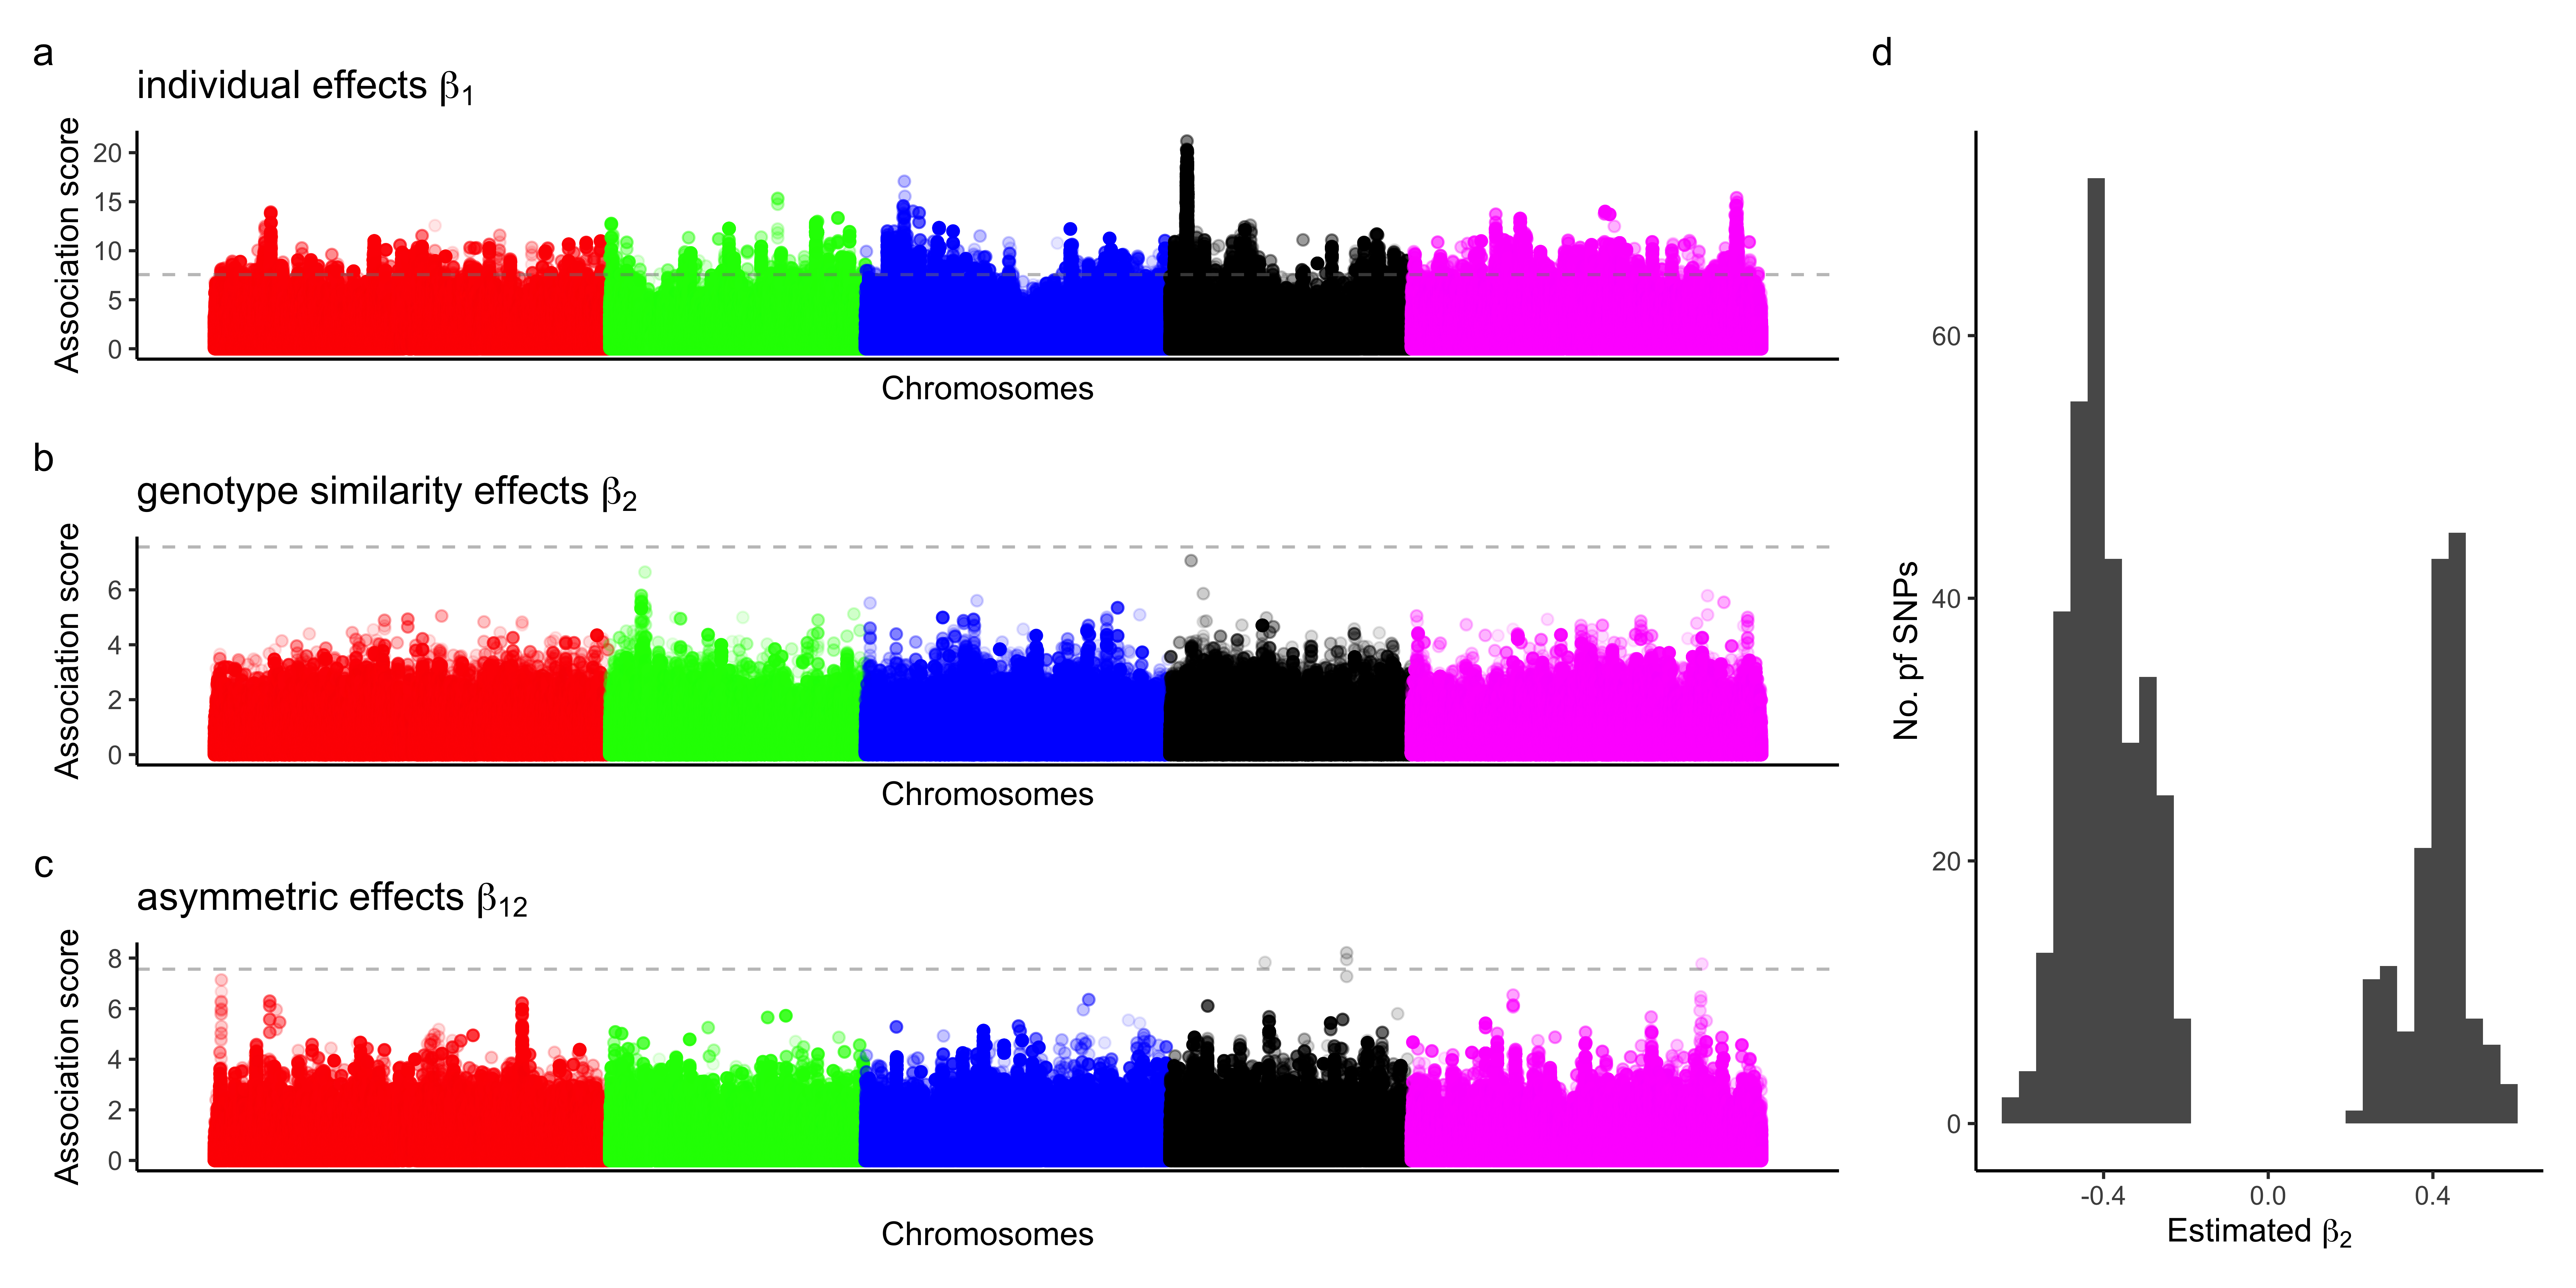
\includegraphics[width=\linewidth]{ManhattanLM.png}
  \caption{Genome-wide association studies of the reproductive branch number in field-grown \textit{A. thaliana}. The results of standard linear models are presented. (a, b, and c) Manhattan plots showing the -log\textsubscript{10}($p$-values) association scores for individual genotype effects, genotype similarity effects, and asymmetric effects, respectively. Horizontal dashed lines indicate $p$-value of $<$ 0.05, after Bonferroni correction. (d) Histogram of estimated $\beta_2$ among single nucleotide polymorphisms (SNPs) exhibiting $p$-values of $< 10^{-4}$. Negative and positive $\beta_2$ infer loci responsible for negative and positive frequency-dependent selection, respectively.}
  \label{figS10:gwasLM}
\end{figure}

\begin{figure}[]
  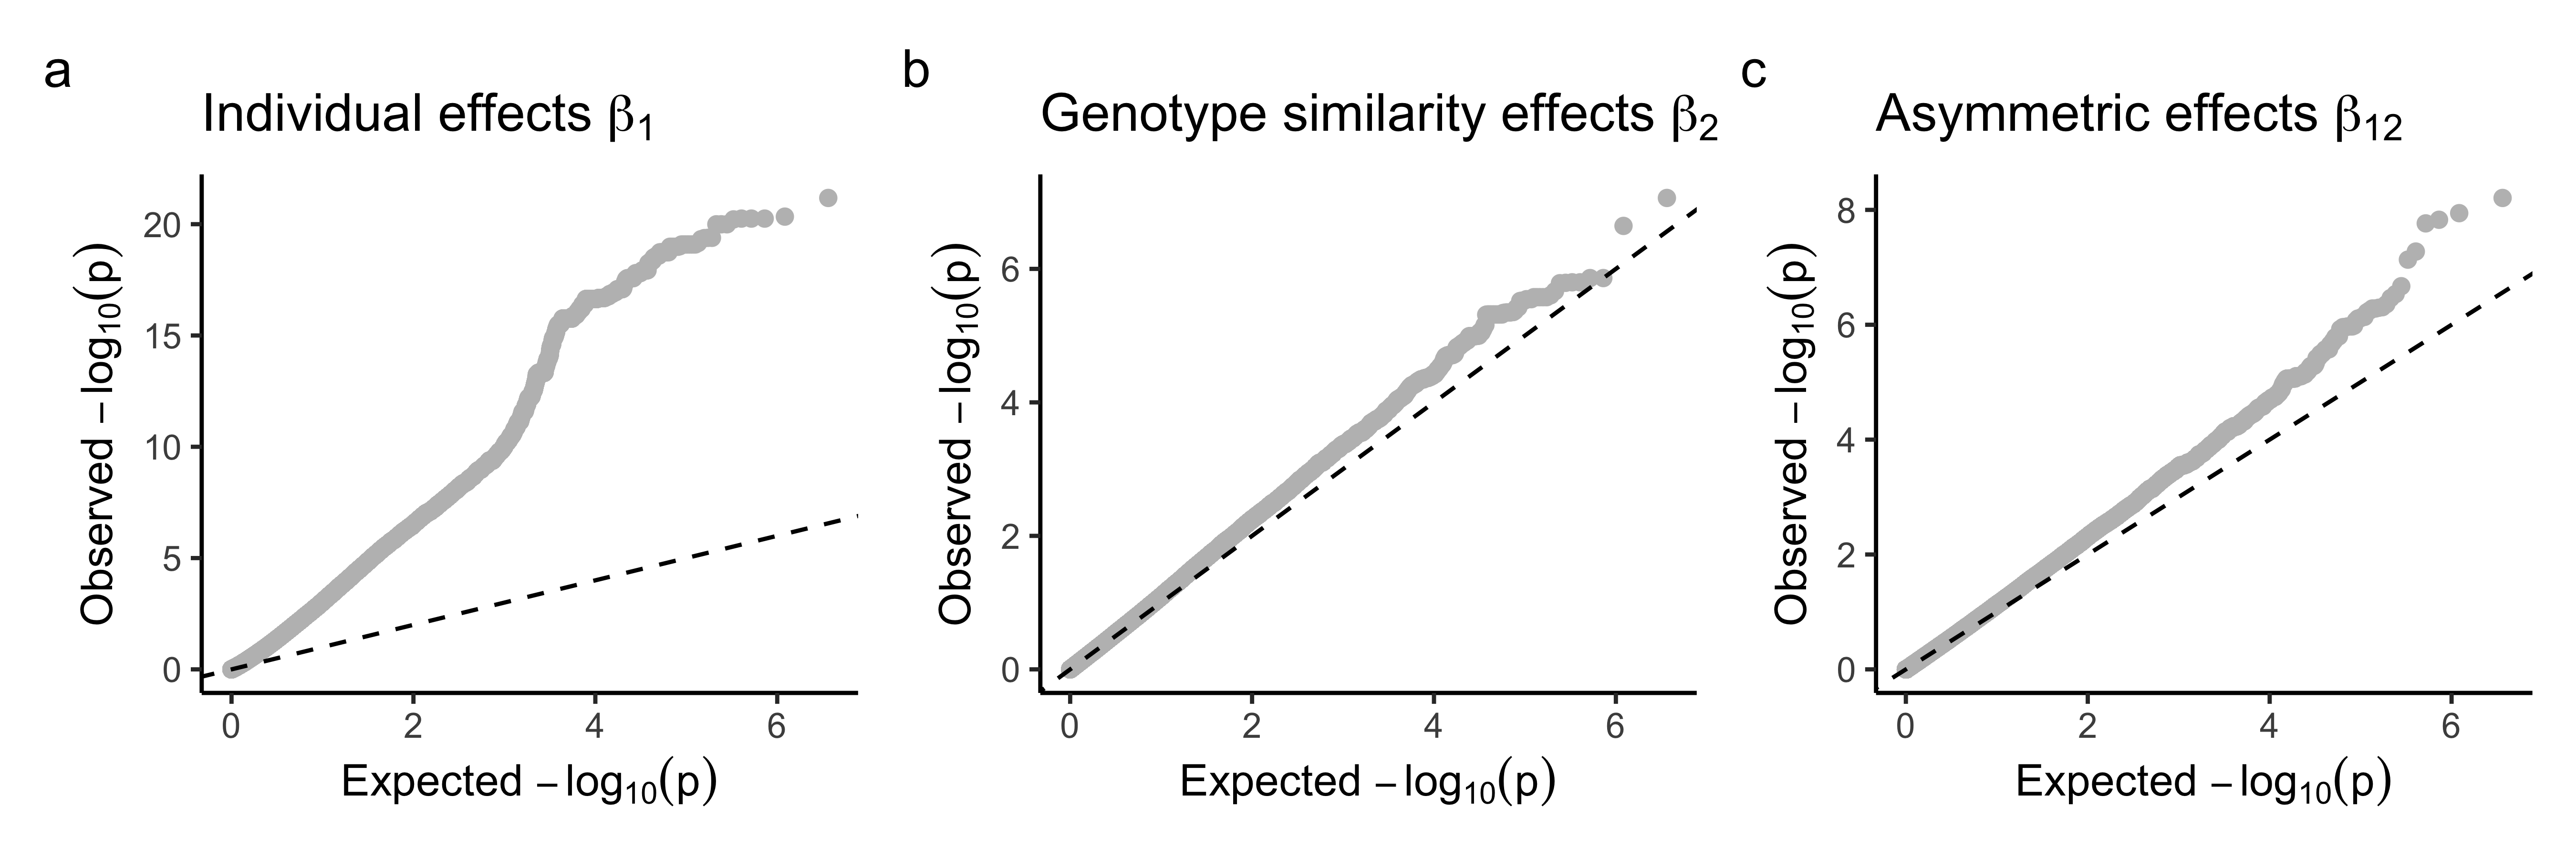
\includegraphics[width=\linewidth]{QQplotLM.png}
  \caption{Quantile-quantile plots showing the observed and expected association score of the -log\textsubscript{10}($p$-values) for the genome-wide association studies of branch number in field-grown \textit{A. thaliana}. The results of standard linear models are presented. The left (a), middle (b), and right (c) panels display individual genotype, genotype similarity, and asymmetric effects, respectively. Dashed lines indicate the identity between the observed and expected association scores.}
  \label{figS11:QQplotLM}
\end{figure}


\newpage
\clearpage
\subsection*{Supplementary Tables S3-S4 (see SuppTablesS3--S4.xlsx)}

\medskip
\noindent
\begin{table}[ht]
\caption{List of plant accessions used for genome-wide association studies (GWAS) and their phenotypes.}
    \label{tableS3:GWASdata}
\end{table}

\medskip
\noindent
\begin{table}[ht]
\caption{List of candidate genes related to individual genotype effects (a), genotype similarity effects (b), and asymmetric effects (c) on the reproductive branch number in \textit{Arabidopsis thaliana}.}
    \label{tableS4:GWAScandidates}
\end{table}

\renewcommand\refname{References}
% This is the default "example" bibtex file which ships with the distribution. Be sure to
% comment out the following line if you want to disable citing all bibtex entries by
% default.
\bibliography{xampl.bib}



\end{document}

%%%%%%%%%%%%%%%%%%%%%%%%%%%%%%%%%%%%%%%%%%%%%%%%%%%%%%%%%%%%%%%%%%%%%%%%%%%%%%
